%%%%%%%%%%%%%%%%%%%%%%%%%%%%%%%%%%%%%%%%%
% The Legrand Orange Book
% LaTeX Template
% Version 1.1 (11/4/13)
%
% This template has been downloaded from:
% http://www.LaTeXTemplates.com
%
% Original author:
% Mathias Legrand (legrand.mathias@gmail.com)
%
% License:
% CC BY-NC-SA 3.0 (http://creativecommons.org/licenses/by-nc-sa/3.0/)
%
% Compiling this template:
% This template uses biber for its bibliography and makeindex for its index.
% This means that to update the bibliography and index in this template you
% will need to run the following sequence of commands in the template
% directory:
%
% 1) pdflatex main
% 2) makeindex main.idx -s StyleInd.ist
% 3) biber main
% 4) pdflatex main
%
% This template also uses a number of packages which may need to be
% updated to the newest versions for the template to compile. It is strongly
% recommended you update your LaTeX distribution if you have any
% compilation errors.
%
% Important note:
% Chapter heading images should have a 2:1 width:height ratio,
% e.g. 920px width and 460px height.
%
%%%%%%%%%%%%%%%%%%%%%%%%%%%%%%%%%%%%%%%%%

%----------------------------------------------------------------------------------------
%	PACKAGES AND OTHER DOCUMENT CONFIGURATIONS
%----------------------------------------------------------------------------------------

\documentclass[11pt,fleqn]{book} % Default font size and left-justified equations

\usepackage[top=3cm,bottom=3cm,left=3.2cm,right=3.2cm,headsep=10pt,a4paper]{geometry} % Page margins

\usepackage{xcolor} % Required for specifying colors by name
\definecolor{ocre}{RGB}{243,102,25} % Define the orange color used for highlighting throughout the book

% Font Settings
\usepackage{avant} % Use the Avantgarde font for headings
%\usepackage{times} % Use the Times font for headings
\usepackage{mathptmx} % Use the Adobe Times Roman as the default text font together with math symbols from the Sym­bol, Chancery and Com­puter Modern fonts
\usepackage{microtype} % Slightly tweak font spacing for aesthetics
\usepackage[utf8]{inputenc} % Required for including letters with accents
\usepackage[T1]{fontenc} % Use 8-bit encoding that has 256 glyphs

% Bibliography
\usepackage{hyperref} %added by GTG
\usepackage{csquotes} %added by GTG
%\usepackage[backend=bibtex]{biblatex} %added by GTG
%\usepackage[sorting=nyt,sortcites=true,autopunct=true,babel=hyphen,hyperref=true,abbreviate=false,backend=biber]{biblatex} %style=alphabetic,backref=true,
%\addbibresource{bibliography.bib} % BibTeX bibliography file
%\defbibheading{bibempty}{}

% Index
%\usepackage{calc} % For simpler calculation - used for spacing the index letter headings correctly
%\usepackage{makeidx} % Required to make an index
%\makeindex % Tells LaTeX to create the files required for indexing

% added by GTG
\usepackage{verbatim}
\usepackage{alltt}
\usepackage{parskip}
\usepackage{paralist}
\usepackage{enumitem}
\usepackage{changepage}
\usepackage[official]{eurosym}
\usepackage{subcaption}
\usepackage{nameref}
\usepackage{wrapfig}
\usepackage{bbm}
\usepackage{listings}

\def\numversion{2.3}
\def\svnversion{R1039}

%----------------------------------------------------------------------------------------

\input{structure} % Insert the commands.tex file which contains the majority of the structure behind the template

\begin{document}

%==============================================================================
% TITLE PAGE
%==============================================================================
\begingroup
\thispagestyle{empty}
\AddToShipoutPicture*{\put(6,5){\includegraphics[scale=1]{background}}} % Image background
\vspace*{-1cm}
\centerline{\includegraphics[angle=0]{./Pictures/logo.png}}
\centering
\vspace*{0.5cm}
\par\normalfont\fontsize{35}{35}\sffamily\selectfont
Credit Risk Modeling \par % Book title
\par\normalfont\fontsize{25}{25}\sffamily\selectfont
Using CCruncher\par
\vspace*{2cm}
{\huge Gerard Torrent-Gironella}\par % Author name
\vspace*{2cm}
\par\normalfont\fontsize{14}{14}\sffamily\selectfont
Version \numversion\par
\endgroup


%==============================================================================
% COPYRIGHT PAGE
%==============================================================================
\newpage

\section*{Acknowledgements}
TODO\@: SET ACKNOWLEDGEMENTS HERE

~\vfill
\section*{Contributors}
Be the first!

~\vfill
The BibTeX entry of this document for \LaTeX\ users is:
%\footnotesize 
\begin{alltt}
@manual\{ccruncher,
    title = \{Credit Risk Modeling Using CCruncher\},
    author = \{Torrent-Gironella, Gerard\},
    organization = \{Tatine\},
    address = \{Barcelona, Catalonia, Spain\},
    year = \{2013\},
    url = \{http://www.ccruncher.net/\},
    edition = \{\numversion\}
\}
\end{alltt}

~\vfill
\thispagestyle{empty}
\noindent Version \numversion\ [\svnversion]\\ 
\\
\noindent Copyright \copyright\ 2013 Gerard Torrent\\
\\
\noindent 
This work is licensed to the public under Creative Commons 
Attribution-ShareAlike 3.0 Unported License. To view a copy 
of this license visit 
\url{http://creativecommons.org/licenses/by-sa/3.0/}.
We have invested a lot of time and effort in creating CCruncher, 
please cite it when using it for credit risk analysis.


%==============================================================================
% TABLE OF CONTENTS
%==============================================================================
\chapterimage{chapter_head_1.pdf} % Table of contents heading image
\pagestyle{empty} % No headers
\setcounter{tocdepth}{1}
\tableofcontents % Print the table of contents itself
\cleardoublepage % Forces the first chapter to start on an odd page so it's on the right
\pagestyle{fancy} % Print headers again


%==============================================================================
% INTRODUCTION
%==============================================================================
\chapter{Introduction}

The \textbf{CCruncher} project provides a framework for quantify portfolio 
credit risk. It is developed and maintained by 
\href{http://www.tatine.es}{Tatine}, a quantitative consulting firm located 
in Barcelona (Catalonia, Spain). You can download the latest version of the 
project from the CCruncher's site, \url{http://www.ccruncher.net}.

The framework consist of this document that explains the models and algorithms, 
and a piece of software that implements it in an efficient way. 
Both elements, documentation and software, are licensed with open-source type 
licenses. CCruncher is a mature and active project in which you can participate 
sending your suggestions and contributions to 
\href{mailto:gtorrent@ccruncher.net}{gtorrent@ccruncher.net}.
Because it is an evolving project, it is recommended to mention the version
identifier when you refer the project name (eg. CCruncher-\numversion).

This document provides a comprehensive view of credit risk modeling 
under the copula approach (t-Student case), emphasizing the practical aspects. 
Care is taken to make short introductions about the methods and concepts used, 
give examples, and to mention the small details of implementation.
This document does not provide new basic results. Most exposed models and 
algorithms are used for some time. There are two exceptions to this. First, 
no references have been found about the internals of parameter estimation
in the general case. For this reason, the development of this section is 
original. Its validity has been verified with tests listed in the document. 
And second, the minor result that states that t-Student multi-factor model 
and multivariate t-Student with correlation block matrix are quasi-equivalents 
when the number of components in each factor are high.

Portfolio credit risk try to respond to questions like: \enquote{what is the 
portfolio expected loss for the next year?}, and \enquote{how much could I 
lose in a really bad year?}. There are several approaches to answer these 
questions. Here we present briefly the two most used approaches~\cite{crouhy:2000} 
\cite[chap. 2.4]{bluhm:2002}. Both try to do the same: obtain the portfolio 
loss distribution and measure the credit risk using a set of selected 
statistics (eg.\ mean, quantile). They differ on how to obtain this 
distribution. 

\textbf{Actuarial approach}. This approach considers that the frequency 
distribution of defaults (Poisson type) is the proper way to interpret the 
observed defaults. Compounding defaults frequency with the obligors' exposures 
gives the portfolio loss distribution that can be approximated by Panjer 
recursion, or by the FFT method. The main representative of this approach is 
the CreditRisk+ model~\cite{creditrisk+:1997}.

\textbf{Merton based approach}. This approach considers that the obligors' 
probabilities of default are the proper way to explain the observed defaults.
The sum of the obligors' exposures weighted by the probabilities of default 
gives the portfolio loss distribution. This distribution is approximated 
using the Monte Carlo method. The main representative of this approach is the 
CreditMetrics\texttrademark~\cite{cmetrics:1997} model. Other representatives 
are the KMV model, or the copula approach~\cite{li:2000}. The Basel II 
accord~\cite{basel2:2006}, the de-facto international financial risk 
regulation framework, is strongly influenced by this 
approach~\cite{cespedes:2002}.

Both approaches give similar results for simple cases~\cite{koyluoglu:1998},
but differ when the dependence structure between obligors is distinct than
the simplistic case~\cite{bluhm:2001}. CCruncher implements the copula 
approach, a Merton model variant that put the focus on the dependence among 
obligors, one of the key points in the credit risk quantification.

\textbf{Copula approach}. This approach considers that the obligors default 
times are the proper way to explain the observed defaults. The dependence 
between these default times is modeled using a copula. The sum of the 
obligors' exposures at the default times gives the portfolio loss distribution.
David X. Li introduced this approach in the famous document
\emph{On Default Correlation: A Copula Function Approach}~\cite{li:2000}
which stated that the CreditMetrics{\texttrademark} model can be interpreted 
in the copula approach context and that has a Gaussian copula.

CCruncher quantify the portfolio credit risk simulating the portfolio loss
distribution multiple times and computing the appropriate statistics (EL, 
VaR, ES) over this sample. The portfolio losses are obtained simulating 
the obligors default times and the EADs and LGDs of its assets. These 
default times are a multivariate distribution where its marginals are 
the probabilities of default given by the obligors ratings, and dependence
structure between obligors are determined by the obligors industrial sector.
CCruncher assumes that the dependence structure is a t-Student copula.
This document provides a guide to estimate the copula parameters using
Bayesian inference and encourages to transfer the parameters uncertainty
to the credit risk measures.

CCruncher quantifies the credit risk of portfolios with a buy-and-hold policy. 
Also it is necessary that each obligor have an assigned rating, belongs to an 
unique economic sector, and has known assets exposures and recoveries. 
An example of a credit portfolio that can benefit of CCruncher is a SMEs 
loan portfolio (buy-and-hold, rated obligors, multiple sectors where each
obligor belongs to a unique sector, known EADs and LGDs).
Unlike CreditMetrics{\texttrademark}, CCruncher don't follows a mark-to-market 
account, but follows a two-state model (default/no-default). Later we use the 
transition matrix concept in order to determine the shape of PD functions, 
not to perform an accounting type mark-to-market.

The advantages of CCruncher are: 
\begin{inparaenum}[1)]
	\item avoids over-simplifications, 
	\item supports multiple risk measures (eg. user defined),
	\item don't presuppose uniform transition matrix,
	\item correlations are considered suitably, 
	\item allows to consider parameters uncertainty,
	\item allows multiple sub-portfolios (risk disaggregation),
	\item allows multiple factors,
	\item allows multiple ratings,
	\item obligors can have multiple assets,
	\item each of them with their own EAD and LGD,
	\item that can be stochastic values, and
	\item vary over the time.
\end{inparaenum}

The disadvantages of CCruncher are: 
\begin{inparaenum}[1)]
	\item computationally intensive,
	\item slow (requires a big amount of simulations),
	\item lack of precision due to Monte Carlo barrier $1/\sqrt{N}$,
	\item obligors can't belong to a weighted sum of factors,
	\item correlations are constants over time,
	\item dependence only rely on sector,
	\item only a copula type is supported, and
	\item mark-to-market not supported.
\end{inparaenum}
Despite this, CCruncher is designed to be very fast doing most simulations
in seconds or minutes if the number of obligors in the portfolio is huge 
(eg.\ 50000).

The content is organized in three chapters. The first one details the 
distribution used to simulate the obligors default times. It is easy to 
understand and is recommended reading, specially the section where is 
related the multivariate model. The second chapter penetrates into
the parameters estimation. This topic can be rough for those not familiarized 
with MCMC, for this reason it includes a detailed introduction to the 
Metropolis-Hastings method. You can skip this chapter if you don't need 
to estimate the parameters of the obligors default times model. Finally, the 
third chapter contains the credit portfolio loss quantification and details 
of the implementation. It is recommended reading. You can skip the last 
section referred to parameters uncertainty if you are not concerned about 
parameters estimation and its impact in the credit risk measures.
There are four little appendices that covers aspects used in the first 
chapter (default times modeling). They are a recommended reading because
contains key statements and establish the used notation.

%TODO: identificar els suposits (cicle econ., rating 1-year, etc.)
%TODO: implications (fixed correlations, economic cycle)


%==============================================================================
% MODELING DEFAULT TIMES
%==============================================================================
\chapter{Modeling Default Times}

The model described in this section is the same as described in 
~\cite{li:2000,roncalli:2001,frey:2001}~\cite[chap. 2.6]{bluhm:2002}.
We recommend taking a look at the appendices before to proceed.
These contain definitions, statements, notation and details about subjects 
used in this chapter.

%------------------------------------------------------------------------------
% THE PROBABILITIES OF DEFAULT
%------------------------------------------------------------------------------
\section{The Probabilities of Default}

\begin{definition}[Probability of Default (PD)]
	The Probability of Default of the i-th obligor, $\text{PD}_i(t)$
	indicates the probability that this obligor defaults in the time 
	interval $(0,t]$.
	\begin{displaymath}
		\text{PD}_i(t) = \Pr\{T_i \le t\} = 
		\Pr\{\text{ i-th obligor defaults before $t$ years }\}
	\end{displaymath}
	where $T_i$ is a random variable that represents the default
	time of the i-th obligor. Note that the PD defined in this way 
	is the cdf of $T_i$. We indicate as $p_i$ the probability that 
	i-th obligor defaults in the time range $[0,1]$.
	\begin{displaymath}
		p_i = \Pr\{T_i \le 1\} = \text{PD}_i(1) 
	\end{displaymath}
	Some texts~\cite{li:2000,roncalli:2001} use the concept of 
	survival instead of the PD\@. The survival is defined as:
	\begin{displaymath}
		\text{Survival}_i(t) = 1-\text{PD}_i(t)
	\end{displaymath}
\end{definition}

Each obligor has its own PD depending on its rating. This causes that 
all obligors with the same rating have the same PD\@. These few PDs can 
be inferred from the transition matrix, the construct that contains the 
relationship between ratings. 
Below show three different ways of inferring the PD depending 
upon the amount of information available. All of them give similar 
results when the time unit and evaluation time is reduced (eg.\ 1 year) 
but differ as this goes away.

\begin{definition}[Transition matrix]
	\label{def:tm}
	The $T$-years transition matrix gives the probability of changing 
	from rating $r_i$ to rating $r_j$ in a period of $T$ years:
	\small
	\begin{displaymath}
		M_T = \left(
		\begin{array}{ccc}
			m_{11} & \cdots & m_{1n} \\
			\vdots & \ddots & \vdots \\
			m_{n1} & \cdots & m_{nn} \\
		\end{array}
		\right)
		\qquad
		m_{ij} = \Pr(r_i \to r_j\ ;\ T)
	\end{displaymath}
	where $n$ is the number of ratings and $m_{ij}$ is the probability that a
	obligor with rating $r_i$ end up having the rating $r_j$ after $T$ years.
	Note that row sums are $1$, and that two consecutives transition matrices, 
	$M_{T_1}$ and $M_{T_2}$, gives $M_{T_1+T_2} = M_{T_1} \cdot M_{T_2}$.
\end{definition}

\begin{example}
	\label{ex:1ytm}
	Table~\ref{tmatrix1} shows a transition matrix, extracted 
	from~\cite[p. 20]{cmetrics:1997}, in which the probability that a obligor 
	with rating AA changes to rating B in one year is $0.14\%$. Note that 
	last column contains the 1-year default probabilities for each rating, and 
	the last row corresponds to the \emph{defaulted} rating.
	\begin{table}[!ht]
		\begin{center}
			\begin{tabular}[]{l|rrrrrrrr}
				        & AAA     & AA      & A       & BBB     & BB      & B                  & CCC     & Default  \\
				\hline
				AAA     & $90.81$ & $8.33$  & $0.68$  & $0.06$  & $0.12$  & $0.00$             & $0.00$  & $0.00$   \\
				AA      & $0.70$  & $90.65$ & $7.79$  & $0.64$  & $0.06$  & $\underline{0.14}$ & $0.02$  & $0.00$   \\
				A       & $0.09$  & $2.27$  & $91.05$ & $5.52$  & $0.74$  & $0.26$             & $0.01$  & $0.06$   \\
				BBB     & $0.02$  & $0.33$  & $5.95$  & $86.93$ & $5.30$  & $1.17$             & $0.12$  & $0.18$   \\
				BB      & $0.03$  & $0.14$  & $0.67$  & $7.73$  & $80.53$ & $8.84$             & $1.00$  & $1.06$   \\
				B       & $0.00$  & $0.11$  & $0.24$  & $0.43$  & $6.48$  & $83.46$            & $4.07$  & $5.21$   \\
				CCC     & $0.22$  & $0.00$  & $0.22$  & $1.30$  & $2.38$  & $11.24$            & $64.86$ & $19.78$  \\
				Default & $0.00$  & $0.00$  & $0.00$  & $0.00$  & $0.00$  & $0.00$             & $0.00$  & $100.00$ \\
			\end{tabular}
			\caption{One-year transition matrix \%}
			\label{tmatrix1}
		\end{center}
	\end{table}
\end{example}

\subsection{From annual PDs}
\label{pdfsv}

In some circumstances the complete transition matrix is not available, 
and we only have the probabilities of default at T-years for each rating, 
$p_1,\dots,p_n$. In the absence of more information, we can considerer 
the following diagonal transition matrix:
\begin{displaymath}
	M_T = \left(
	\begin{array}{cccc}
		1-p_1  & \cdots & 0         & p_1     \\
		\vdots & \ddots & \vdots    & \vdots  \\
		0      & \cdots & 1-p_{n-1} & p_{n-1} \\
		0      & \cdots & 0         & 1       \\
	\end{array}
	\right)
\end{displaymath}

We can derive the PDs from this matrix applying the following 
section~\ref{pdftm}, but this simplified case has an explicit
solution stated in the proposition that follows.

\begin{proposition}
	A diagonal transition matrix as above leads to default times with 
	exponential distributions:
	\begin{displaymath}
		\Pr\{T_. \le t\} = 1 - e^{-\lambda t} 
		\quad \text{ where } \lambda = -\ln(1-p_j)
	\end{displaymath}
\end{proposition}
\begin{proof}
	We note that ratings are detached from each other. 
	For this reason we do the proof for a generic rating and we
	use the subscripts to indicate the time, not the rating.
	Let $p_t$ the probability of default in the time range $[0,t]$ and
	$q_t=1-p_t$ the probability of survival. We express $p_1$ in term
	of $p_{\frac{1}{n}}$ using the geometric serie formula.
	\begin{displaymath}
		p_1 = p_{\frac{1}{n}} \cdot q_{\frac{1}{n}}^{(n-1)} + 
			p_{\frac{1}{n}} \cdot q_{\frac{1}{n}}^{(n-2)} + \cdots + 
			p_{\frac{1}{n}} \cdot q_{\frac{1}{n}} + 
			p_{\frac{1}{n}}
		= p_{\frac{1}{n}} \cdot \frac{1-q_{\frac{1}{n}}^n}{1-q_{\frac{1}{n}}}
		= 1 - q_{\frac{1}{n}}^n
		= 1- (1-p_{\frac{1}{n}})^n
	\end{displaymath}
	This gives:
	\begin{displaymath}
		p_{\frac{1}{n}} = 1-(1-p_1)^{\frac{1}{n}}
	\end{displaymath}
	We use the limit definition of the logarithm function, that is 
	$\ln(x)=\lim_{n \to \infty} n \cdot(x^{\frac{1}{n}}-1)$, to
	found the following limit:
	\begin{displaymath}
		\lim_{n \to \infty} n \cdot p_{\frac{1}{n}} = 
		\lim_{n \to \infty} -n \cdot ((1-p_1)^{\frac{1}{n}} -1) =
		-\ln(1-p_1) = \lambda
	\end{displaymath}
	We use this equivalence and the limit definition of the 
	exponential function to determine the survival probability:
	\begin{displaymath}
		(1-p_1)^t 
		= \left( \lim_{n \to \infty} (1-p_{\frac{1}{n}})^n \right)^t
		= \left(\lim_{n \to \infty} (1-\frac{\lambda}{n})^n \right)^t
		= e^{-\lambda t}
	\end{displaymath}
	Then,
	\begin{displaymath}
		\Pr\{T_. \le t\} = \text{PD}(t) = 
		1 - \text{Survival}(t) = 1 - e^{-\lambda t}
	\end{displaymath}
\end{proof}

If $T$ is a reduced time horizon (eg.\ 1 year) then the linear function
can be a good-enough approximation. To see this we use the Taylor series
of the exponential and the logarithm functions:
\begin{displaymath}
	\begin{array}{l}
		e^x = 1 +x + \frac{x^2}{2!} + \frac{x^3}{3!} + \dots
		\\
		\ln(1-x) = -x - \frac{x^2}{2} - \frac{x^3}{3} + \dots
		\\
		\Pr\{T. \le t\} = 1-e^{-\lambda\cdot t} \approx
		1 - (1-\lambda \cdot t) = \lambda \cdot t = 
		- \ln(1-p) \cdot t \approx p \cdot t
	\end{array}
\end{displaymath}

\begin{example}
	\label{ex:pdfsv}
	Suppose that we only know the ratings annual probabilities of default 
	and that these values are those from the 1-year regularized transition 
	matrix of example~\ref{ex:1ytm}. In this case, the diagonal transition 
	matrix is:
	{\small
	\begin{displaymath}
		M_1 = \left(
		\begin{array}{cccccccc}
		99.9991 & 0 & 0 & 0 & 0 & 0 & 0 & 0.0009 \\
		0 & 99.9923 & 0 & 0 & 0 & 0 & 0 & 0.0077 \\
		0 & 0 & 99.9400 & 0 & 0 & 0 & 0 & 0.0600 \\
		0 & 0 & 0 & 99.8200 & 0 & 0 & 0 & 0.1800 \\
		0 & 0 & 0 & 0 & 98.9401 & 0 & 0 & 1.0599 \\
		0 & 0 & 0 & 0 & 0 & 94.7997 & 0 & 5.2003 \\
		0 & 0 & 0 & 0 & 0 & 0 & 80.2154 & 19.7846 \\
		0 & 0 & 0 & 0 & 0 & 0 & 0 & 100 \\
		\end{array}
		\right)
	\end{displaymath}\par}
	We determine the PDs function for each rating using the 
	proposition~\ref{prop:pdftm}, that is, considering that default times are 
	exponential distributions. Results are displayed in figure~\ref{fig:pdfsv}. 
	Observe that values around $T=1$ are similar to those of 
	example~\ref{ex:pdftm}, but they differ as they move away from this.
	\begin{figure}[!ht]
		\centering
		\subcaptionbox{Probability of Default}{
			\includegraphics[width=7cm]{pdfsv1}
		}
		\subcaptionbox{Probability of Default (zoom)}{
			\includegraphics[width=7cm]{pdfsv2}
		}
		\caption{PDs derived from annual PDs}
		\label{fig:pdfsv}
	\end{figure}
\end{example}

\subsection{From transition matrix}
\label{pdftm}

This approach implies that transition probabilities remains constant
over time undermining the economic cycle effect. In practice, it is 
equivalent to consider an averaged economic cycle.

\begin{proposition}[Scaled transition matrix]
	The transition matrix can be scaled in time by using the following rules:
	\begin{itemize}
		\item $M_{k \cdot T} = M_{T}^k$
		\item $M_{\frac{T}{k}} = \sqrt[k]{M_{T}}$
	\end{itemize}
\end{proposition}

The root of a matrix $M$ can be obtained using the spectral decomposition
$M = P \cdot D \cdot P^{-1}$, where $P$ and $D$ are the eigenvectors and
eigenvalues matrices of $M$, doing $M^{\gamma} = P \cdot D^{\gamma} \cdot P^{-1}$

Sometimes, the scaled transition matrix does not satisfy the Markov conditions
(the row sum is equal to one, and all elements are non-negatives). In this case, 
we need to transform this matrix to the relevant Markov matrix. This process is 
called regularization. Below is exposed the QOM regularization algorithm 
extracted from~\cite{kreinin:2001}.

\begin{algorithm}[Transition matrix regularization]
	The QOM (Quasi-Optimization of the root Matrix) algorithm regularizes a 
	$n {\times} n$ transition matrix $M$, row by row. The steps to 
	regularize the $i$-th row are:
	\begin{enumerate}
		\item Compute the difference between the row sum and one. 
		Divide by $n$ and subtract this value from all non-zero components:
		\begin{displaymath}
			m_{ij} \ne 0 
			\Longrightarrow 
			m_{ij} = m_{ij} - \frac{1}{n} \left( \sum_{k=1}^{n} m_{ik} - 1\right)
		\end{displaymath}
		\item If all the row elements are non-negative and sum to one, 
		then stop, as the row is regularized.
		\item Fix any negative row element to zero and go to Step 1.
	\end{enumerate}
	
	Apply the previous algorithm for every row. The algorithm stops after $m$ 
	steps, where $m \le n$ (Merkoulovitch 2000). The final matrix is a regularized
	matrix. 
\end{algorithm}

\begin{proposition}[PDs derived from transition matrix]
	\label{prop:pdftm}
	Let $M_T$ a transition matrix, then the PD for an obligor with 
	rating $r_j$ is:
	\begin{displaymath}
		\Pr\{T_. \le t\} = \left( M_t \right)_{jn}
	\end{displaymath}
	where $T_.$ is the obligor default time, $j$ is the index of the obligor's
	rating, $n$ is the index of the \emph{defaulted} rating, $M_t$ is the 
	transition matrix scaled to time $t$, and $(M)_{ij}$ is the matrix element
	in the i-th row and j-th column.
\end{proposition}

\begin{example}
	\label{ex:pdftm}
	We derive the PD for each rating induced by the transition matrix exposed
	in the example~\ref{ex:1ytm}. As first step, we scale the 1-year transition 
	matrix $M_1$ to the 1-month transition matrix $M_{\frac{1}{12}}$.
	{\small
	\begin{displaymath}
		M_{\frac{1}{12}} = \left(
		\begin{array}{cccccccc}
			99.1972 &  0.7588 &  0.0320 &  0.0020 &  0.0112 & -0.0011 & -0.0001 &   0.0000 \\
			 0.0635 & 99.1744 &  0.7083 &  0.0392 &  0.0015 &  0.0120 &  0.0018 &  -0.0007 \\
			 0.0074 &  0.2057 & 99.1980 &  0.5102 &  0.0557 &  0.0189 & -0.0001 &   0.0042 \\
			 0.0014 &  0.0239 &  0.5507 & 98.8021 &  0.5164 &  0.0871 &  0.0077 &   0.0106 \\
			 0.0027 &  0.0113 &  0.0396 &  0.7581 & 98.1557 &  0.8774 &  0.0889 &   0.0665 \\
			-0.0007 &  0.0098 &  0.0196 &  0.0111 &  0.6447 & 98.4443 &  0.4463 &   0.4240 \\
			 0.0233 & -0.0023 &  0.0170 &  0.1287 &  0.2166 &  1.2298 & 96.4213 &   1.9667 \\
			 0.0000 &  0.0000 &  0.0000 &  0.0000 &  0.0000 &  0.0000 &  0.0000 & 100 \\
		\end{array}
		\right)
	\end{displaymath}\par}
	We observe that $M_{\frac{1}{12}}$ is not a regular matrix due to negative
	values. We apply the QOM algorithm to regularize it. We call the 1-year 
	regularized transition matrix to $\bar{M}_1 = \bar{M}_{\frac{1}{12}}^{12}$.
	{\small
	\begin{displaymath}
		\bar{M}_{\frac{1}{12}} = \left(
		\begin{array}{cccccccc}
			99.1969 &  0.7586 &  0.0317 &  0.0018 &  0.0110 &  0.0000 &  0.0000 &   0.0000 \\
			 0.0634 & 99.1744 &  0.7082 &  0.0391 &  0.0014 &  0.0119 &  0.0017 &   0.0000 \\
			 0.0074 &  0.2057 & 99.1980 &  0.5102 &  0.0557 &  0.0189 &  0.0000 &   0.0041 \\
			 0.0014 &  0.0239 &  0.5507 & 98.8021 &  0.5164 &  0.0871 &  0.0077 &   0.0106 \\
			 0.0027 &  0.0112 &  0.0395 &  0.7581 & 98.1557 &  0.8774 &  0.0889 &   0.0665 \\
			 0.0000 &  0.0099 &  0.0197 &  0.0111 &  0.6447 & 98.4444 &  0.4463 &   0.4240 \\
			 0.0228 &  0.0000 &  0.0165 &  0.1282 &  0.2161 &  1.2293 & 96.4208 &   1.9663 \\
			 0.0000 &  0.0000 &  0.0000 &  0.0000 &  0.0000 &  0.0000 &  0.0000 & 100 \\
		\end{array}
		\right)
	\end{displaymath}\par}
	Finally we use the proposition~\ref{prop:pdftm} to determine the 
	PD function for each rating and month. Results are displayed in 
	figure~\ref{fig:pdftm}.
	\begin{figure}[!ht]
		\centering
		\subcaptionbox{Probability of Default}{
			\includegraphics[width=7cm]{pdftm1}
		}
		\subcaptionbox{Probability of Default (zoom)}{
			\includegraphics[width=7cm]{pdftm2}
		}
		\caption{PDs derived from transition matrix}
		\label{fig:pdftm}
	\end{figure}
\end{example}

\subsection{From advanced models}

There are financial institutions that may have models to forecast 
the transition matrix using some economic indicators like GDP
or inflation. We note as $M_T(t)$ the T-period transition matrix
at time $t$. This matrix depends of the forecasted indicators at 
$t$ in the form $M_T(\theta_1(t),\dots,\theta_k(t))$. In these 
cases, the PDs functions can be obtained composing successively
the transition matrices for each T-period. The PD for an obligor
with rating $r_j$ is:
\begin{displaymath}
	\Pr\{T_. \le t\} = \left(
		\left( \prod_{i=1}^{[t/T]} M_T(i) \right) \cdot 
		M_{t-T\cdot[t/T]}\left([t/T]+1\right) 
		\right)_{jn}
\end{displaymath}
where $[x]$ is the integer part of $x$, $T_.$ is the obligor default time, 
$j$ is the index of the obligor's rating, $n$ is the index of the 
\emph{defaulted} rating, $M_t(i)$ is the T-period transition matrix 
evaluated at time $i$ and scaled to time $t$, and $(M)_{ij}$ is the 
matrix element in the i-th row and j-th column.

The PDs functions derived from an advanced transition matrix model may 
have more or less pronounced steps depending on the different stages of 
the economic cycle. This approach is the most suitable for risk estimates 
in the medium and long term.

Finally, there may be models that do not come from a transition matrix.
CCruncher allows to describe the PD for each rating specifying its value
at given time points. These have to meet the cdf conditions:
\begin{itemize}
	\item $\text{PD}_r(0) = 0$,
	\item strictly increasing, 
	\item $\text{PD}_r(\infty) = 1$, and
	\item $\text{PD}_{\text{default}}(t) = 1 \quad \forall\ t \ge 0$.
\end{itemize}
The functions specified in this way are interpolated using cubic splines
when the above conditions are preserved or linear splines when not.

%------------------------------------------------------------------------------
% THE MULTIVARIATE MODEL
%------------------------------------------------------------------------------
\section{The Multivariate Model}

\subsection{The copula approach}
The copula approach considers that the obligors default times are the 
proper way to explain the observed defaults. This default times 
$(T_1, \dots, T_n)$ are modeled by a multivariate distribution $F$ 
such that:
\begin{displaymath}
	F(t_1, \dots, t_n) = \Pr \{T_1 \le t_1, \dots, T_n \le t_n\}
\end{displaymath}
where $n$ is the number of obligors in the portfolio, $T_i$ is the time 
(in years) when the i-th obligor defaults, and $F$ is the multivariate
default times distribution. Applying the Sklar's theorem to the above 
distribution we obtain:
\begin{displaymath}
	F(t_1, \dots, t_n) = 
	C\left(\text{PD}_1(t_1), \dots, \text{PD}_n(t_n)\right)
\end{displaymath}
where marginal $\text{PD}_i(t) = \Pr\{T_i \le t\}$ is the Probability 
of Default of the i-th obligor, and $C$ is a copula. There are several 
proposals on the copula to be used. CCruncher considers that it is a 
t-Student copula for the following reasons:

\begin{itemize}
	\item is determined by the correlation matrix (elliptical). 
	\item is symmetrical (elliptical), allowing to 
	apply the antithetic reduction variance technique in the Monte Carlo 
	simulation.
	\item allows a wide range of dependence structures through parameter $\nu$.
	\item it exhibits tail dependence when $\nu \ne \infty$.
	\item exist an efficient simulation algorithm.
	\item the Gaussiana case ($\nu = \infty$) is the copula used by 
	CreditMetrics\texttrademark.
	\item it can be expressed as a multi-factor model.
\end{itemize}

Previous versions of the CCruncher project implemented a simulation schema
consisting in simulating the t-Student copula directly. This approach 
requires an adapted simulation algorithm for high-dimensional problems~\cite{torrent:2012}
and difficult the estimation of the parameters. The current CCruncher version 
relies in the following proposition that reformulate $F$ in terms of the 
multivariate t-Student distribution. This result, combined with the t-Student
multi-factor model, provides an efficient simulation algorithm and allows 
estimating the parameters.

\begin{proposition}[Multivariate Default Times Distribution]
	\label{prop:dtd}
	Let $T=(T_1,\dots,T_n)$ the obligors default times with marginals 
	$\text{PD}_i$ and a t-Student copula $C_{\nu,\bar{R}}^n$ with $\nu$
	degrees of freedom and a $n {\times} n$ obligors correlation matrix 
	$\bar{R}$. Then, its distribution $F$ is:
	\begin{displaymath}
		F(t_1,\dots,t_n) = H\left(t_\nu^{-1}(\text{PD}_1(t_1)), \dots, t_\nu^{-1}(\text{PD}_n(t_n))\right)
	\end{displaymath}
	where $H$ is the cdf of the multivariate t-Student distribution 
	$t_n(\nu,0,\bar{R})$, and $t_\nu^{-1}$ is the inverse of the univariate 
	t-Student distribution $t_1(\nu,0,1)$.
\end{proposition}
\begin{proof}
	We note as $X=(X_1,\dots,X_n)$ a vector having a multivariate t-Student
	distribution $t_n(\nu,\bar{R})$, and $(U_1,\dots,U_n)$ to represent
	the components of the copula $C_{\nu,\bar{R}}^n$.
	\begin{displaymath}
		\begin{array}{rl}
			F(t_1,\dots,t_n) = & \Pr\{ T_1 \le t_1 , \dots, T_n \le t_n \} =                                    \\
			                   & \text{we use the corollary~\ref{cor:cop3}: }                                   
			(T_1,\dots,T_n) = (\text{PD}_1^{-1}(U_1),\dots,\text{PD}_n^{-1}(U_n)) \\
			=                  & \Pr\{ \text{PD}_1^{-1}(U_1) \le t_1 , \dots , \text{PD}_n^{-1}(U_n) \le t_n \} =               \\
			                   & \text{we use the corollary~\ref{cor:cop2}: }                                   
			(U_1,\dots,U_n) = (t_\nu(X_1),\dots,t_\nu(X_n)) \\
			=                  & \Pr\{ \text{PD}_1^{-1}(t_\nu(X_1)) \le t_1 , \dots , \text{PD}_n^{-1}(t_\nu(X_n)) \le t_n \} = \\
			=                  & \Pr\{ t_\nu(X_1) \le \text{PD}_1(t_1) , \dots , t_\nu(X_n) \le \text{PD}_n(t_n) \} =           \\
			=                  & \Pr\{ X_1 \le t_\nu^{-1}(\text{PD}_1(t_1)) , \dots , X_n \le t_\nu^{-1}(\text{PD}_n(t_n)) \} = \\
			=                  & H(t_\nu^{-1}(\text{PD}_1(t_1)), \dots, t_\nu^{-1}(\text{PD}_n(t_n)))                           \\
		\end{array}
	\end{displaymath}
\end{proof}

The previous proposition can be stated by any other copula coming from
a multivariate distribution an applied if this had a known distribution 
and marginals (eg.\ the Gaussian copula). Also from the previous proposition
is immediate to derive a method to sample the default times distribution.

\begin{corollary}[Default times simulation (I)]
	\label{cor:dts1}
	Let $T=(T_1, \dots, T_n)$ a random vector with marginals 
	$\text{PD}_1, \dots, \text{PD}_n$ and a t-Student copula $C_{\nu,\bar{R}}^n$. 
	Then we can simulate this distribution using a multivariate t-Student 
	distribution $X \sim t_n(\nu,\bar{R})$:
	\begin{displaymath}
		(T_1, \dots, T_n) = \left(\text{PD}_1^{-1}\left(t_{\nu}(X_1)\right), \dots, \text{PD}_n^{-1}\left(t_{\nu}(X_n)\right)\right)
	\end{displaymath}
\end{corollary}

The current formulation is not yet satisfactory because the dimension 
$n {\times} n$ of the obligors correlation matrix causes that any 
operation (eg.\ simulate random value, or estimate the parameters) cannot 
be done in practice when $n$ is large. For this reason we introduce the
multi-factor formulation.

\subsection{The multi-factor formulation}

To bypass the dimension problem we assuming that exist a reduced number 
$k$ of industrial sectors and that each obligor belong to a unique sector. 
Also that default times dependence between obligors only depends on the 
involved industrials sectors. With these restrictions, if we sort the 
obligors by sector, the obligors default times correlation matrix, $\bar{R}$, 
is a $n {\times} n$ correlation block matrix $B_k(\vec{n},\vec{1},M)$. See 
appendix~\ref{ap:cbm} for more information about covariance block matrices. 
\begin{displaymath}
	\bar{R} = B_k(\vec{n},\vec{1},M) = 
	\left(
	\begin{array}{ccccccc}
		1         & \cdots & \rho_{11} &        & \rho_{1k} & \cdots & \rho_{1k} \\
		\vdots    & \ddots & \vdots    & \cdots & \vdots    &        & \vdots    \\
		\rho_{11} & \cdots & 1         &        & \rho_{1k} & \cdots & \rho_{1k} \\
		
		          & \vdots &           & \ddots &           & \vdots &           \\
		
		\rho_{1k} & \cdots & \rho_{1k} &        & 1         & \cdots & \rho_{kk} \\
		\vdots    &        & \vdots    & \cdots & \vdots    & \ddots & \vdots    \\
		\rho_{1k} & \cdots & \rho_{1k} &        & \rho_{kk} & \cdots & 1         \\
	\end{array}
	\right)
	\qquad 
	\begin{array}{l}
		M = 
		\left(
		\begin{array}{ccc}
		\rho_{11} & \cdots & \rho_{1k} \\
		\vdots    & \ddots & \vdots    \\
		\rho_{1k} & \cdots & \rho_{kk}
		\end{array}
		\right) \\
		\\
		\vec{n} = (n_1,\dots,n_k)
	\end{array}
\end{displaymath}

Up to this point the multivariate default times distribution $F$ can 
be expressed by its marginals $\text{PD}_i$ and a multivariate t-Student 
distribution, $t_n(\nu,0,\bar{R})$ with a obligors correlation block 
matrix $\bar{R} = B_k(\vec{n},\vec{1},M)$. The proposition that follows 
gives us the key to reformulate the problem as a multi-factor problem.

\begin{proposition}[t-Student distr.\ as a multi-factor model]
	\label{prop:tmfm}
	Let a random vector $X=(X_1,\dots,X_n)$ with a multivariate t-Student 
	distribution $t_n(\nu,0,\bar{R})$ where $\bar{R} = B_k(\vec{n},\vec{1},M)$ 
	is a correlation block matrix and $n_i$ sizes are high-enough. 
	Then $X$ can be written as a t-Student multi-factor model as follows:
	\begin{displaymath}
		X_i^j = \sqrt{\frac{\nu}{V}} \cdot 
		\left( w_i \cdot Z_i + \sqrt{1-w_i^2} \cdot \epsilon_i^j \right)
		\text{, where } \left\{
		\begin{array}{l}
			i = 1, \dots, k \quad \text{ and $k$ is the number of blocks}      \\
			j = 1, \dots, n_i \quad \text{ and $n_i$ is i-th block size}       \\
			V \sim \chi_{\nu}^2, \quad 2 \le \nu \text{ degrees of freedom}    \\
			Z \sim N(0,R), \text{ and $R$ a $k {\times} k$ correlation matrix} \\
			w_i \in (0,1), \text{ are the factor loadings }                    \\
			\epsilon_i^j \sim N(0,1) \text { iid } \forall\ i,j                \\
			V, Z, \epsilon_i^j \text{ independents } \forall\ i,j              \\
		\end{array}
		\right.
	\end{displaymath}
	where $w_1,\dots,w_k$ and $R$ satisfy:
	\begin{displaymath}
		\begin{array}{l}
			R_{ii} = 1 \quad i = 1,\dots,k \\
			M_{ij} = w_i \cdot w_j \cdot R_{ij} \quad \forall\ i,j
		\end{array}
	\end{displaymath}
\end{proposition}
\begin{proof}
	We use the t-Student characterization (proposition~\ref{prop:mtschar}),
	$X = \sqrt{\frac{\nu}{V}} \cdot Z$, where $V \sim \chi_{\nu}^2$ and 
	$Z \sim N(0,\bar{R})$ expressing $Z$ as a Gaussian multi-factor model 
	(definition~\ref{def:gmfm}). The determination of $R$ and $w_1,\dots,w_n$
	values can be found at proposition~\ref{prop:gmfigs}. The tag line 
	\enquote{$n_i$ sizes are high-enough} is justified in 
	proposition~\ref{prop:gmfamgb}.
\end{proof}

Note that we expressed the multi-factor model in terms of the factor 
loadings and the factors correlation matrix, instead of the more concise 
covariance matrix. We do this because the factor loadings have a treatment 
distinct than factors correlation in the estimation of parameters.

Factor loadings $\vec{w}$, measures the correlation between obligors 
belonging the same industrial sector $i$, satisfying in the Gaussian case 
that $\rho_i = w_i^2$. Factor correlations $R$ measures the correlation 
between factors, and also the correlation between obligors belonging to 
different sectors, satisfying in the Gaussian case that 
$\rho_{ij} = w_i \cdot w_j \cdot R_{ij}$.

The t-Student multi-factor model combined with the corollary~\ref{cor:dts1} 
provides an efficient algorithm to simulate the obligors default times.

\begin{corollary}[Default times simulation (II)]
	\label{cor:dts2}
	Let $T=(T_1, \dots, T_n)$ a random vector with marginals 
	$\text{PD}_1, \dots, \text{PD}_n$ and a t-Student copula $C_{\nu,\bar{R}}^n$
	coming from a t-Student multi-factor model with $\nu$ degrees of freedom, 
	factor loadings $\vec{w}$, and factor correlations $R$. Then we can simulate 
	this distribution doing:
	\begin{enumerate}
		\item Simule the factors, $\vec{z} \sim N(0,R)$.
		\item Simule the degrees of freedom, $\nu \sim \chi_{\nu}^2$.
		\item For each obligor repeat the following steps:
		\begin{enumerate}
			\item Simule $\epsilon \sim N(0,1)$.
			\item Simule the multivariate t-Student component using the obligor's sector:
			\begin{displaymath}
				x = \sqrt{\frac{\nu}{v}} \cdot \left( w_s \cdot z_s + \sqrt{1-w_s^2} \cdot \epsilon \right)
			\end{displaymath}
			\item Obtain the obligor's default time using the obligor's rating:
			\begin{displaymath}
				t = \text{PD}_r^{-1}\left(t_{\nu}(x)\right)
			\end{displaymath}
		\end{enumerate}
	\end{enumerate}
\end{corollary}


%==============================================================================
% ESTIMATING PARAMETERS
%==============================================================================
\chapter{Estimating Parameters}

We want to estimate the dependence parameters of the multivariate default 
times model. These are the degrees of freedom $\nu$, the factor loadings 
$\vec{w}$, and the factors correlation matrix $R$ of the multi-factor 
formulation.

\begin{definition}[Annual number of defaults]
	We define the annual number of defaults by sector and rating like a
	discrete multivariate random variable $K=(K_{11}, \dots, K_{sr})$ where:
	\begin{displaymath}
		K_{ij} = \left\{
		\begin{array}{c}
			\text{number of defaults in the sector $i$ in a period of} \\
			\text{1-year having a rating $j$ at the beginning of the period}
		\end{array}
		\right\}
	\end{displaymath}
	taking in account that:
	\begin{displaymath}
		N_{ij} = \left\{
		\begin{array}{c}
			\text{number of obligors in the sector $i$ in a period of} \\
			\text{1-year having a rating $j$ at the beginning of the period}
		\end{array}
		\right\}
	\end{displaymath}
	Note that $K_{ij} \le N_{ij}$. We use the superscript to indicate 
	the observation at time $t$, $N_{ij}^t$ and $K_{ij}^t$. 
	%When the subscript only has one index ($K_{i}$ and $N_{i}$) this means 
	%that values are aggregated by sector. 
\end{definition}

% It is possible that the there is no historical records disaggregated at 
% the rating level. In these cases, when the historical records are 
% $\left\{N_{s}^t, K_{s}^t \right\}_{t=1,\dots,T}$ without the counts by 
% rating, we can use the following approximation:
% \begin{displaymath}
	% K_{ij}^t = K_{i}^t \cdot \frac{\lambda_{ij}^t \cdot p_j}{\displaystyle \sum \lambda_{ik}^t \cdot p_k}
	% \quad \text{ where }
	% \lambda_{ij}^t \approx \frac{\text{\# obligors sector $i$ rating $j$}}{\text{\# obligors sector $i$}}
% \end{displaymath}
% Values $\lambda_{ij}^t$ depends on the characteristics of the portfolio 
% and the economic cycle and requires to be estimated based on historical 
% data and current PD models.

We provide an algorithm to simulate the number of defaults based on
the multi-factor model. We will use it to generate samples with which 
we can test the estimation algorithm. The following algorithm is 
a direct application of the multivariate default times distribution
and the t-Student multi-factor model (see propositions~\ref{prop:dtd} 
and~\ref{prop:tmfm}).

\begin{algorithm}[Simulating number of defaults]
	\label{alg:snod}
	Let a multivariate default times distribution with a t-Student copula
	that has $k$ factors, factor loadings $\vec{w}$, factors correlation 
	matrix $R$, degrees of freedom $\nu$, and annual probabilities of
	default $p_j$ where $j=1,\dots,m$. Then, we can simulate a sample of 
	size $T$ of the annual number of defaults by factor and rating doing:
	\begin{enumerate}
		\item Compute the Cholesky decomposition of R, $R = L \cdot L^\intercal$
		\item For $t=1,\dots,T$ repeat the following steps
		\begin{itemize}
			\item Simulate $k$ independent $N(0,1)$, $\vec{z}$
			\item Simulate factors doing $\vec{z} = L \cdot \vec{z}$
			\item Simulate a $\chi_{\nu}^2$, $v$
			\item For $i=1,\dots,k$ and $j=1,\dots,m$ repeat the following steps
			\begin{itemize}
				\item Simulate $n_{ij}$ independent $N(0,1)$, $\vec{\epsilon}$
				\item Compute $\vec{x} = \sqrt{\frac{\nu}{v}} \cdot \left( w_i \cdot z_i + \sqrt{1-w_i^2} \cdot \vec{\epsilon} \right)$
				\item $k_{ij} = \left\{ \text{number of components of $\vec{x}$ less than $t_{\nu}^{-1}(p_j)$} \right\} $
			\end{itemize}
		\end{itemize}
	\end{enumerate}
\end{algorithm}

\begin{example}[]
	We have two sectors, S1 and S2, and four ratings, A, B, C, D, where 
	D is the defaulted status. We have collected the observations displayed
	in table~\ref{table:histdata}.
	This example has a number of ratings and sectors less than the previous 
	examples for practical reasons (otherwise data tables do not fit 
	in the width of the page).
	\begin{table}[!ht]
		\centering
		\begin{tabular}{cc|c|c|c||c|c|c|  c  |c|c|c||c|c|c|}
			\cline{3-8} \cline{10-15}
			& & \multicolumn{6}{|c|}{N (\# obligors)} & & \multicolumn{6}{|c|}{K (\# defaults)} \\
			\cline{3-8} \cline{10-15}
			& & \multicolumn{3}{|c||}{S1} & \multicolumn{3}{|c|}{S2} & & \multicolumn{3}{|c||}{S1} & \multicolumn{3}{|c|}{S2} \\
			\cline{1-1} \cline{3-8} \cline{10-15}
			\multicolumn{1}{|c|}{Year} & & A & B & C & A & B & C & & A & B & C & A & B & C \\
			\cline{1-1} \cline{3-8} \cline{10-15}
			\multicolumn{1}{|c|}{1} & & 529 & 932 & 293 & 685 & 1249 & 206 & & 3 & 12 & 15 & 3 & 25 & 10 \\
			\cline{1-1} \cline{3-8} \cline{10-15}
			\multicolumn{1}{|c|}{2} & & 522 & 977 & 278 & 638 & 1315 & 194 & & 1 & 18 & 13 & 7 & 28 & 8 \\
			\cline{1-1} \cline{3-8} \cline{10-15}
			\multicolumn{1}{|c|}{\vdots} & & \vdots & \vdots & \vdots & \vdots & \vdots & \vdots & & \vdots & \vdots & \vdots & \vdots & \vdots & \vdots \\
			\cline{1-1} \cline{3-8} \cline{10-15}
			\multicolumn{1}{|c|}{20} & & 492 & 962 & 310 & 602 & 1227 & 183 & & 6 & 28 & 21 & 4 & 31 & 16 \\
			\cline{1-1} \cline{3-8} \cline{10-15}
		\end{tabular}
		\caption{Example of historical records}
		\label{table:histdata}
	\end{table}
\end{example}

%------------------------------------------------------------------------------
% DISTRIBUTION OF THE NUMBERS OF DEFAULTS
%------------------------------------------------------------------------------
\section{Distribution of the Number of Defaults}

Before proceeding to estimate the parameters, we need to know the density
of the number of observed defaults in order to define a likelihood 
function. In this section we derive this distribution from the multivariate
default times distribution. More info at~\cite{gordy:2002,roncalli:2004}.

\begin{proposition}[Density of the annual number of defaults (I)]
	The density of the annual number of defaults, assuming that default 
	times are distributed according to a multivariate block t-Student distribution
	with $\nu$ degrees of freedom, and $n {\times} n$ obligors block correlation 
	matrix $\bar{R} = B_k(\vec{n},\vec{1},M)$, is:
	\begin{displaymath}
		\begin{array}{l}
			K(k_{11},\dots,k_{sr}\ ;\ \nu, \bar{R}) = 
			\Pr\{K_{11}=k_{11},\dots,K_{sr}=k_{sr}\ ;\ \nu, \bar{R}\} = \\
			\\
			= \left( \displaystyle \prod_{i=1}^s \prod_{j=1}^r \binom{n_{ij}}{k_{ij}} \right) \cdot       
			\displaystyle                                                                                 
			\underbrace{\int_{-\infty}^{t_{\nu}^{-1}(p_1)}}_{k_{11} \text{ times}}                        
			\underbrace{\int_{t_{\nu}^{-1}(p_1)}^{\infty}}_{n_{11}-k_{11} \text{ times}}                  
			\dots                                                                                         
			\underbrace{\int_{-\infty}^{t_{\nu}^{-1}(p_r)}}_{k_{sr} \text{ times}}                        
			\underbrace{\int_{t_{\nu}^{-1}(p_r)}^{\infty}}_{n_{sr}-k_{sr} \text{ times}}                  
			f(x_1,\dots,x_n)\ \ud x_1 \dots \ud x_n                                                        
		\end{array}
	\end{displaymath}
	where $n_{ij}$ and $k_{ij}$ are respectively the number of obligors and 
	defaults in the i-th sector with the j-th rating, $p_j = \text{PD}_j(1)$ 
	is the probability to default in 1-year of the j-th rating, $f(\vec{x})$ 
	is the pdf of $t_n(\nu,\bar{R})$, and $t_{\nu}^{-1}$ is the inverse of the 
	cdf of the univariate t-Student. The combinatorial coefficients take in 
	account all the combinations of exchangeable obligors.
\end{proposition}

We don't know an analytical expression for the density of the annual number 
of defaults. Furthermore, the numerical solution of the integral is difficult 
when the number of obligors is larger than a few. For this reason we try 
to solve the problem recurring to the multi-factor formulation.

\begin{proposition}[Conditioned density of the annual number of defaults]
	The conditioned density of the annual number of defaults, assuming 
	that default times are distributed according to a t-Student multi-factor 
	model with $\nu$ degrees of freedom, factor loadings $\vec{w}$, and 
	factors correlations $R$ is:
	\begin{displaymath}
		\begin{array}{l}
			K(k_{11},\dots,k_{sr} \mid v,\vec{z}\ ;\ \nu,\vec{w}, R) = 
			\Pr\{K_{11}=k_{11},\dots,K_{sr}=k_{sr} \mid v,\vec{z}\ ;\ \nu, \vec{w}, R\} = \\
			                                                                                                                                 \\
			= \displaystyle \prod_{i=1}^s \prod_{j=1}^r \binom{n_{ij}}{k_{ij}} \cdot
			H_{ij}(v,z_i)^{k_{ij}} \cdot
			\left( 1 - H_{ij}(v,z_i) \right)^{n_{ij}-k_{ij}}
		\end{array}
	\end{displaymath}
	where
	\begin{displaymath}
		H_{ij}(v,z_i) = \phi\left(  
		\frac{\sqrt{\frac{v}{\nu}} \cdot t_{\nu}^{-1}(p_j) - w_i\cdot z_i}{\sqrt{1-w_i^2}}
		\right)
	\end{displaymath}
	and $n_{ij}$ and $k_{ij}$ are respectively the number of obligors and 
	defaults in the i-th sector with the j-th rating, $p_j = \text{PD}_j(1)$ 
	is the probability to default in 1-year of the j-th rating,
	$\phi$ is the pdf of the univariate $N(0,1)$, and $t_{\nu}^{-1}$ is the 
	inverse of the cdf of the univariate t-Student. The combinatorial coefficients 
	take in account all the combinations of exchangeable obligors.
\end{proposition}
\begin{proof}
	Let $H_{ij}$ the probability that an obligor belonging to sector $i$
	with initial rating $j$ defaults the first year conditioned to $z_i$ 
	and $v$. We use the pdf of the default times distribution (see 
	proposition~\ref{prop:dtd}) to assess it value:
	\begin{displaymath}
		H_{ij}(v,z_i) = 
		\Pr\{T_k \le 1 \mid v, z_i\} = 
		\Pr\{ X_k \le t_{\nu}^{-1}(\text{PD}_j(1)) \mid v, z_i\} = 
		\Pr\{ X_k \le t_{\nu}^{-1}(p_j) \mid v, z_i\}
	\end{displaymath}
	where the k-th obligor belongs to sector $i$ and has rating $j$, 
	$T_k$ is the k-th component of the multivariate default 
	times, and $X_k$ is the k-th component of the multivariate t-Student. 
	Now express $X$ in the multi-factor form:
	\begin{displaymath}
		H_{ij}(v,z_i) = \Pr \left\{ 
		\sqrt{\frac{\nu}{v}} \cdot \left( w_i \cdot z_i + \sqrt{1-w_i^2} \cdot \epsilon\right)
		\le t_{\nu}^{-1}(p_j) \mid v, z_i
		\right\}
	\end{displaymath}
	Because $v$ and $z_i$ are fixed and independent from $\epsilon \sim N(0,1)$, we obtain:
	\begin{displaymath}
		H_{ij}(v,z_i) = \phi\left(  
		\frac{\sqrt{\frac{v}{\nu}} \cdot t_{\nu}^{-1}(p_j) - w_i\cdot z_i}{\sqrt{1-w_i^2}}
		\right)
	\end{displaymath}
	Once the probability of default by one obligor, the probability of 
	observing $k_{ij}$ failures in a set of $n_{ij}$ independent obligors 
	follows a binomial distribution with default probability $H_{ij}$:
	\begin{displaymath}
		\text{Bin}(k_{ij}\ ;\ n_{ij},H_{ij}) = 
		\binom{n_{ij}}{k_{ij}} \cdot H_{ij}^{k_{ij}} \cdot (1-H_{ij})^{n_{ij}-k_{ij}}
	\end{displaymath}
	The product for all sectors and ratings gives the stated formula. 
	We can do the product because $v$ and $z_i$ are fixed.
\end{proof}

\begin{corollary}[Density of the annual number of defaults (II)]
	We can express the density of the annual number of defaults using 
	the conditioned density:
	\begin{displaymath}
		\begin{array}{l}
			K(k_{11},\dots,k_{sr}\ ;\ \nu, \vec{w}, R) =                \\
			\\
			\displaystyle \int_0^{\infty} \int_{\mathbb{R}^k}                                         
			\psi(v) \cdot \phi(\vec{z}) \cdot
			K(k_{11},\dots,k_{sr} \mid v,\vec{z}\ ;\ \nu,\vec{w}, R) 
			\ \ud z_1 \dots \ud z_k \ud v
		\end{array}
	\end{displaymath}
	where $\psi$ is the pdf of $\chi_{\nu}^2$, and $\phi$ is the pdf of $N(0,R)$.
\end{corollary}

This expression has a dimension significantly less than before, but like 
that, it hasn't a known analytical expression and it can't be approximated 
numerically with accuracy when the number of factors is high (eg. 10).


%------------------------------------------------------------------------------
% BAYESIAN INFERENCE
%------------------------------------------------------------------------------
\section{Bayesian Inference}

\begin{wrapfigure}{r}{0.4\textwidth}
	\vspace{-20pt}
	\begin{center}
		\includegraphics[width=0.38\textwidth]{ccbnd}
	\end{center}
	\vspace{-10pt}
	\caption{Distr.\ of correlation coefficient of the bivariate Normal with $\rho=0.2$ and sample size $20$.}
	\vspace{-10pt}
	\label{fig:ccbnd}
\end{wrapfigure}
Parameters $\vec{w}$ and $R$ are variances and correlations that must be 
estimated. It is difficult to estimate this type of statistics. To illustrate
this we suppose a simplified problem: estimate the correlation of a bivariate 
Normal distribution with $\rho=0.2$ from a sample size of $20$. 
Figure~\ref{fig:ccbnd} displays the distribution of the correlation 
coefficient~\cite[pp. 217--221]{kenney:1951}. We observe that the 
uncertainty is important. In fact, the probability that we observe a negative 
correlation coefficient is significant despite having a correlation value as 
high as $0.2$. Our goal is the inverse case, we have a correlation coefficient 
from a sample size of $20$ observations and we estimate the original $\rho$.
The previous observation about the dispersion indicates that the 
searched value will also can have an important dispersion.
This is exacerbated by the fact that some of our variables
are latent, and that we are estimating from observations of type
count-data. After this, considering the estimated parameters as 
unique values, like the Maximum Likelihood estimator, is a naive and 
risky positioning. The Bayesian approach seems  more appropriate 
\cite{gossl:2005,tarashev:2010} because it takes into account 
the uncertainty of the parameters. Later we will see how to transfer 
this uncertainty to the assessment of credit risk.

Bayesian statistics differ from the classical statistical 
theory since all unknown parameters are considered as random 
variables. We want calculate the distribution $f(\theta \mid y)$ 
of the parameters $\theta$ given the observed data $y$. 
According to the Bayes theorem, this can be written as:
\begin{displaymath}
	f(\theta \mid y) = \frac{f(y \mid \theta) \cdot f(\theta)}{f(y)} \propto f(y \mid \theta) \cdot f(\theta)
\end{displaymath}

We call \emph{posterior distribution} to $f(\theta \mid y)$ and 
\emph{prior distribution} to $f(\theta)$. This prior distribution 
expresses the information available to the researcher before 
any data are involved in the statistical analysis. $f(y \mid \theta)$ 
is the probability of observing $y$ given $\theta$, and is also 
known as the likelihood.
\begin{displaymath}
	f(y \mid \theta) = \prod_{i=1}^n f(y_i \mid \theta)
\end{displaymath}

In our case, we can define an analytic likelihood function using the 
conditional density of the number of defaults. Thus it implies that 
the parameters to be inferred are $\nu,\vec{w},R$ and the latent 
variables $v^1,\vec{z}^1,\dots,v^T,\vec{z}^T$.

\begin{definition}[Conditioned likelihood]
Let a set of observations $\{K^t, N^t\}_{t=1,\dots,T}$ where $N^t$ 
and $K^t$ are vectors representing the number of obligors and defaulted 
obligors in each sector-rating bucket. We define the conditional 
likelihood of these observations as:
\begin{displaymath}
	\begin{array}{l}
		L(\nu,\vec{w},R \mid v^1,\vec{z}^1,\dots,v^T,\vec{z}^T\ ;\ K^1,\dots,K^T) = \\
		\displaystyle \prod_{t=1}^T K(k_{11}^t,\dots,k_{sr}^t \mid v^t,\vec{z}^t\ ;\ \nu,\vec{w},R) = \\
		\displaystyle
		\prod_{t=1}^T \prod_{i=1}^s \prod_{j=1}^r 
		\binom{n_{ij}^t}{k_{ij}^t} \cdot
		H_{ij}(v^t,z_i^t)^{k_{ij}^t} \cdot
		\left( 1 - H_{ij}(v^t,z_i^t) \right)^{n_{ij}^t-k_{ij}^t}
	\end{array}
\end{displaymath}
\end{definition}

%------------------------------------------------------------------------------
% METROPOLIS-HASTINGS ALGORITHM
%------------------------------------------------------------------------------
\section{Metropolis-Hastings Algorithm}

This section contains a brief introduction to Bayesian inference using the 
Metropolis-Hastings algorithm and it is heavily influenced by the book 
\emph{Bayesian Modeling Using WinBUGS}~\cite{ntzoufras:2009}.

When doing Bayesian inference we can find a closed-form of the posterior 
distribution only in a very few cases. Usually this has to be determined 
by numerical methods. One of the most used is the Metropolis-Hastings 
algorithm that belongs to the family of Markov Chain Monte Carlo (MCMC) 
methods. These are based on the construction of a Markov chain that converges 
to the target distribution which, in our case, is the posterior distribution.

\begin{definition}[Markov chain]
	A Markov chain is a stochastic process 
	$\left\{\theta^{(1)},\theta^{(2)},\dots,\theta^{(T)}\right\}$ such that
	\begin{displaymath}
		f\left(\theta^{(t+1)} \mid \theta^{(t)},\dots,\theta^{(1)}\right) = 
		f\left(\theta^{(t+1)} \mid \theta^{(t)}\right)
	\end{displaymath}
	that is, the distribution of $\theta$ at sequence $t+1$ given all the 
	preceding $\theta$ values depends only on the previous value. 
	When the Markov chain is irreducible, aperiodic, and positive-recurrent, 
	as $t \to \infty$ the distribution of $\theta^{(t)}$ converges to its 
	equilibrium distribution, which is independent of the initial values 
	of the chain $\theta^{(0)}$.
\end{definition}

The Markov chain is not a strange concept to us because the transition 
matrix (see definition~\ref{def:tm}) is a Markov chain where its 
equilibrium state is the \emph{defaulted} rating (that is, just any 
obligor ends up defaulting) allowing us to consider the PDs as cdfs.
The Metropolis-Hastings algorithm generates a sample from $f(\theta)$ 
by constructing a Markov chain that has $f(\theta)$ as the equilibrium 
distribution.

\begin{algorithm}[Metropolis-Hastings (M-H)]
	Let us assume a target distribution $f(x)$ from which we wish to 
	generate a sample of size $T$. The Metropolis-Hastings algorithm can 
	be described by the following iterative steps; where $x^{(t)}$ is the 
	vector of generated values in the $t$-th iteration:
	\begin{enumerate}
		\item Set initial values $x^{(0)}$
		\item For $t=1,\dots,T$ repeat the following steps
		\begin{itemize}
			\item Set $x=x^{(t-1)}$
			\item Let $x'$ a random value from the proposal distribution $q(x \to x')=q(x' \mid x)$
			\item Calculate the acceptance rate 
			$\alpha = \min\left(1,\frac{f(x') \cdot q(x \mid x')}{f(x) \cdot q(x' \mid x)}\right)$
			\item Update $x^{(t)}=\left\{
			\begin{array}{ll}
				x'        & \text{ with probability } \alpha   \\
				x^{(t-1)} & \text{ with probability } 1-\alpha 
			\end{array}\right.$ 
		\end{itemize}
	\end{enumerate}
\end{algorithm}

As this is a Markov chain, it is irrelevant the chosen starting point 
$x^{(0)}$ because the algorithm converges to the target distribution
whatever the starting point. If the starting point has low probability 
respect the target distribution, then the initial samples don't come 
from the equilibrium distribution and need to be discarded until it is 
not reached. We call \emph{burnin period} the first $B$ iterations 
eliminated from the sample for this reason.

\textbf{Bayesian inference}.
The Metropolis-Hastings algorithm outlined above can be directly implemented to do
Bayesian inference by substituting $x$ by the unknown parameters, $\theta$, and 
the target distribution $f(x)$ by the posterior distribution $f(\theta \mid y)$. Then 
the acceptance rate becomes:
\begin{displaymath}
	\alpha = \min\left(1,\frac{f(\theta' \mid y) \cdot q(\theta \mid \theta')}{f(\theta \mid y) \cdot q(\theta' \mid \theta)}\right) = \min\left(1,\frac{f(y \mid \theta') \cdot f(\theta') \cdot q(\theta \mid \theta')}{f(y \mid \theta)  \cdot f(\theta) \cdot q(\theta' \mid \theta)}\right)
\end{displaymath}

\textbf{Random-walk Metropolis-Hastings} is a special case with symmetric proposals
$q(\theta' \mid \theta) = q(\theta \mid \theta')$ where $q(\theta' \mid \theta) \equiv N(\theta,\sigma)$. 
In this case the acceptance rate depends only on the posterior distribution
and, in the Bayesian inference Metropolis-Hastings case, becomes:
\begin{displaymath}
	\alpha = 
	\min\left(1,\frac{f(y \mid \theta') \cdot f(\theta') \cdot q(\theta \mid \theta')}{f(y \mid \theta)  \cdot f(\theta) \cdot q(\theta' \mid \theta)}\right) = 
	\min\left(1,\frac{f(y \mid \theta') \cdot f(\theta')}{f(y \mid \theta) \cdot f(\theta)}\right)
\end{displaymath}

The random-walk fixes the shape of the proposal distribution and requires 
specifying the value $\sigma$. This value has a direct non-linear impact 
on the acceptance ratio (\#accepted/\#iterations). Exists an optimal 
acceptance ratio that minimizes the auto-correlation, and in most cases 
relies in the interval $[0.234,0.44]$. To avoid the  manual tuning of the 
scale parameter $\sigma$ we use the Robbins-Monro algorithm~\cite{garthwaite:2010} 
that performs an adaptive scaling to achieve the desired acceptance ratio.

\begin{proposition}[Robbins-Monro process]
	In order to achieve an acceptance ratio $p$ in the random-walk 
	Metropolis-Hastings algorithm, consider the following adaptive
	procedure:
	\begin{displaymath}
		\sigma^{(t+1)} = \left\{
		\begin{array}{ll}
			\sigma^{(t)} \cdot \left( 1 + \frac{1}{p \cdot t} \right) & \text{if $\theta'$ is accepted} \\
			\sigma^{(t)} \cdot \left( 1 - \frac{1}{(1-p) \cdot t} \right) & \text{if $\theta'$ is rejected} \\
		\end{array}
		\right.
	\end{displaymath}
	were the starting value $\sigma_1$ has an arbitrary value.
\end{proposition}

\textbf{Metropolis-Hastings using logarithms}.
The product of functions involves complicated expressions and accuracy 
problems. For this reason it is usual to operate with logarithms. The 
logarithmic version of the acceptance rate, in the Bayesian inference 
Metropolis-Hastings case, becomes:
\begin{displaymath}
	\begin{array}{rl}
		\ln(\alpha) = & \min \left( \ln(1),  
		\ln \left(\frac{f(y \mid \theta') \cdot f(\theta')}{f(y \mid \theta) \cdot f(\theta)}\right)
		\right) = \\
		= & \min \left( 0,
		\ln f(y \mid \theta') + \ln f(\theta') - \ln f(y \mid \theta) - \ln f(\theta)
		\right)
	\end{array}
\end{displaymath}

\textbf{Single-component Metropolis-Hastings} algorithm consists in updates 
sequentially univariate components using Metropolis-Hastings steps. 
One generated observation $\theta^{(t)}$ is obtained after updating all 
components of the parameter vector. Generally, the sequence of updating the 
elements of $\theta$ does not influence the convergence of the algorithm.
Nevertheless, to ensure randomness it is recommended a random selection of 
the updating sequence. We use the notation $\theta_{\backslash j}$ to indicate 
the vector $\theta$ excluding its j-th component [ $\theta_{\backslash j}
= (\theta_1,\dots,\theta_{j-1},\theta_{j+1},\dots,\theta_{d})$ ].

\begin{algorithm}[Bayesian inference Metropolis-Hastings] 
	\label{alg:bimh}
	Let $f(y \mid \theta)$ the likelihood function, with priors $f_j(\theta_j)$,
	and desired acceptance ratios $p_j$. Then the parameters distribution
	can be sampled using the following Metropolis-Hastings algorithm:
	\begin{enumerate}
		\item Set initial values $\theta^{(0)}$
		\item Set initial values $\sigma^{(0)}$
		\item For $t=1,\dots,T$ repeat the following steps
		\begin{itemize}
			\item Set $\theta=\theta^{(t-1)}$
			\item Shuffle update sequence
			\item For $j=1,\dots,d$ repeat the following steps
			\begin{enumerate}[label=\alph*.]
				\item $\theta_j' = N(\theta_j,\sigma_j)$
				\item Calculate the logarithm of the acceptance rate \\
				$\ln(\alpha) = 
					\ln f(y \mid \theta_j',\theta_{\backslash j}) + 
					\ln f_j(\theta_j'\ ;\ \theta_{\backslash j}) - 
					\ln f(y \mid \theta_j,\theta_{\backslash j}) - 
					\ln f_j(\theta_j\ ; \ \theta_{\backslash j})
				$
				\item Simulate $u \sim U(0,1)$
				\item Update $\theta_j=\left\{
				\begin{array}{ll}
					\theta_j' & \text{ if } \ln(u) < \ln(\alpha) \\
					\theta_j  & \text{ otherwise }               
				\end{array}\right.$ 
				\item Update $\sigma_j^{(t)} = \left\{
					\begin{array}{ll}
						\sigma_j^{(t-1)} \cdot \left( 1 + \frac{1}{p_j \cdot t} \right) & \text{ if } \ln(u) < \ln(\alpha) \\
						\sigma_j^{(t-1)} \cdot \left( 1 - \frac{1}{(1-p_j) \cdot t} \right) & \text{ otherwise } \\
					\end{array}
				\right.$
			\end{enumerate}
			\item Set $\theta^{(t)}=\theta$
		\end{itemize}
	\end{enumerate}
\end{algorithm}

The simulated values from the posterior distribution have ergodic properties but
they aren't independents. If you want independent values you can plot the 
autocorrelation function and estimate the length, $B$, for which the autocorrelation 
is canceled. Then take only the values whose index is a multiple of $B$. Also
note that the estimated parameters aren't independent of each other, in fact 
they form a multivariate distribution.

\begin{example}[Beta distribution calibration]
	We have a sample $\{y_1,\dots,y_{100}\}$ coming from a $\text{Beta}(2,5)$ 
	distribution. We want to do Bayesian inference to determine the value of the 
	parameters $\alpha$ and $\beta$ using the Metropolis-Hastings algorithm exposed 
	above. The density of the Beta distribution is:
	\begin{displaymath}
		f(x\ ;\ \alpha, \beta) = 
		\frac{\Gamma(\alpha+\beta)}{\Gamma(\alpha) \cdot \Gamma(\beta)} 
		\cdot x^{(\alpha-1)} \cdot (1-x)^{(\beta-1)}
	\end{displaymath}
	Then, the log-likelihood function is:
	\begin{displaymath}
		\ln f(y \mid \alpha, \beta) = 
		\displaystyle \sum_{i=1}^{100} 
		\ln \Gamma(\alpha+\beta) - \ln \Gamma(\alpha) - \ln \Gamma(\beta) +
		(\alpha-1) \cdot \ln(y_i) + (\beta-1) \cdot \ln(1-y_i)
	\end{displaymath}
	We know that $\alpha \in (0,10)$ and $\beta \in (0,30)$. For this reason we 
	consider that prior distributions $f_{\alpha}()$ and $f_{\beta}()$ are 
	uniform distributions. Then,
	\begin{displaymath}
		\begin{array}{l}
			\ln f_{\alpha}(\alpha \ ;\ \beta) = \ln(\frac{1}{10})
			\\
			\ln f_{\beta}(\beta \ ;\ \alpha) = \ln(\frac{1}{30})
		\end{array}
	\end{displaymath}
	We apply the algorithm~\ref{alg:bimh} with starting point 
	$\left(\alpha^{(0)},\beta^{(0)}\right)=(1,1)$ and 
	desired acceptance ratios $(p_{\alpha},p_{\beta})=(0.3,0.3)$.
	Figure~\ref{fig:mhbd} display the results after 25000 iterations.
	Observe that the first 500 iterations aren't valid because the Markov 
	chain hasn't achieved the equilibrium distribution. These have to be 
	considered into the burnin period. The histogram of the sampled values
	approximates the parameters distribution that we are inferring.
	\begin{figure}[!ht]
		\centering
		\subcaptionbox{Iterations 1--1000 of parameters $\alpha$ and $\beta$}{
			\includegraphics[width=0.98\textwidth]{mhbd1}
		}
		\\
		\subcaptionbox{Histogram parameter $\alpha$}{
			\includegraphics[width=7cm]{mhbd3}
		}
		\subcaptionbox{Histogram parameter $\beta$}{
			\includegraphics[width=7cm]{mhbd4}
		}
		\\
		\subcaptionbox{Iterations 1--1000 of scales $\sigma_{\alpha}$ and $\sigma_{\beta}$}{
			\includegraphics[width=0.98\textwidth]{mhbd2}
		}
		\caption{Metropolis-Hastings algorithm example}
		\label{fig:mhbd}
	\end{figure}
	%TODO: listing R script of this example?
\end{example}

%------------------------------------------------------------------------------
% ESTIMATION OF PARAMETERS
%------------------------------------------------------------------------------
\section{Estimation of Parameters}

\begin{proposition}[Parameters estimation]
	\label{prop:pemh}
	We can estimate the parameters of the conditioned likelihood using
	the Bayesian framework and Metropolis-Hastings algorithm 
	(see algorithm~\ref{alg:bimh}) with the following rules:
	\begin{itemize}
		\item parameters $\theta \equiv \{ \nu,\vec{w},R,v^1,\vec{z}^1,\dots,v^T,\vec{z}^T\}$
		\item observations $y \equiv \{K^t, N^t\}_{t=1,\dots,T}$
		\item likelihood $f(y \mid \theta) \equiv L(\nu,\vec{w},R  \mid  v^1,\vec{z}^1,\dots,v^T,\vec{z}^T\ ;\ K^1,\dots,K^T)$
		\item proposal distributions $q_j(\theta_j \mid \theta_j') \sim N(\theta,\sigma_j)$
		\item prior distribution $f_{\nu}(\nu) \sim \text{Unif}(2,1000)$
		\item prior distribution $f_{w}(w_i) \sim \text{Unif}(0,1) \quad i=1,\dots,k$
		\item prior distribution $f_{r}(r_{ij}\ ;\ R) \sim \Upsilon(\vec{z}^1,\dots,\vec{z}^T,R) \quad i=1,\dots,k, \quad j=(i+1),\dots,k$
		\item prior distribution $f_z(\vec{z}^t\ ;\ R) \sim N(\vec{0},R) \quad t=1,\dots,T$
		\item prior distribution $f_v(v^t) \sim \chi_{\nu}^2 \quad t=1,\dots,T$
	\end{itemize}
	For the prior distributions of $r_{ij}$ we set the likelihood distribution
	of the latent variables $\vec{z}^t$. The pdf of the distribution 
	$\Upsilon(\vec{z}^1,\dots,\vec{z}^T,R)$ is:
	%hyperparameters, hyperdistributions
	\begin{displaymath}
		f_r(r_{ij}\ ;\ R) = \frac
		{\displaystyle \prod_{t=1}^{T} \phi\left( \vec{z}^t\ ;\ \vec{0}, R(r_{ij},i,j) \right)}
		{\displaystyle \int \prod_{t=1}^{T} \phi\left( \vec{z}^t\ ;\ \vec{0}, R(s,i,j) \right) \ud s}
	\end{displaymath}
	where $\phi$ is the pdf of the multivariate $N(0,R)$ distribution,
	and $R(r,i,j)$ is the matrix $R$ with the cell $(i,j)$ value 
	replaced by $r$. We don't need to know the limits of the integral
	because this is constant and cancels into the M-H algorithm.
\end{proposition}

\begin{example}[Model parameters estimation]
	\label{ex:calib}
	Let consider the following scenario:
	\begin{itemize}
		\item t-Student copula with $\nu=20$.
		\item Three ratings \{A, B, D\} where D is the defaulted status, and three 
		sectors \{S1, S2, S3\}, having the following 1-year probabilities of 
		default, factor loadings, and factors correlation matrix:
		\begin{displaymath}
			\begin{array}{l}
				p_A=2\%     \\
				p_B=8\%     \\
			\end{array}
			\quad
			\vec{w} = (0.4, 0.25, 0.3)
			\quad 
			R = \left(
			\begin{array}{ccc}
				1 & 0.5 & 0.3 \\
				0.5 & 1 & 0.4 \\
				0.3 & 0.4 & 1 \\
			\end{array}
			\right) 
		\end{displaymath}
		\item The number of obligors by sector-rating is:\\
		\newline
		\hspace*{1cm}
		\small
		\begin{tabular}{cc|c|c||c|c||c|c|}
			\cline{3-8}
			& & \multicolumn{6}{|c|}{N (\# obligors)} \\
			\cline{3-8}
			& & \multicolumn{2}{|c||}{S1} & \multicolumn{2}{|c||}{S2} & \multicolumn{2}{|c|}{S3} \\
			\cline{1-1} \cline{3-8}
			\multicolumn{1}{|c|}{Obs} & & A & B & A & B & A & B \\
			\cline{1-1} \cline{3-8}
			\multicolumn{1}{|c|}{1} & & 250 & 750 & 500 & 500 & 750 & 250 \\
			\cline{1-1} \cline{3-8}
			\multicolumn{1}{|c|}{2} & & 250 & 750 & 500 & 500 & 750 & 250 \\
			\cline{1-1} \cline{3-8}
			\multicolumn{1}{|c|}{\vdots} & & \vdots & \vdots & \vdots & \vdots & \vdots & \vdots \\
			\cline{1-1} \cline{3-8}
			\multicolumn{1}{|c|}{1000} & & 250 & 750 & 500 & 500 & 750 & 250 \\
			\cline{1-1} \cline{3-8}
		\end{tabular}
	\end{itemize}
	\vspace{11pt}

	\textbf{1000 observations}. We simulate 1000 observations of the numbers of 
	defaults by sector-rating using the algorithm~\ref{alg:snod}. Then we infer 
	the parameters distribution from this sample using the Metropolis-Hastings 
	algorithm~\ref{alg:bimh}. Results are displayed in figure~\ref{fig:calib1}.
	Note that variance of factor loadings is lower than factor correlations.
	\begin{figure}[!ht]
		\centering
		\subcaptionbox{Simulated defaults}{
			%\small
			\begin{tabular}{cc|c|c||c|c||c|c|}
				\cline{3-8}
				& & \multicolumn{6}{|c|}{K (\# defaults)} \\
				\cline{3-8}
				& & \multicolumn{2}{|c||}{S1} & \multicolumn{2}{|c||}{S2} & \multicolumn{2}{|c|}{S3} \\
				\cline{1-1} \cline{3-8}
				\multicolumn{1}{|c|}{Obs} & & A & B & A & B & A & B \\
				\cline{1-1} \cline{3-8}
				\multicolumn{1}{|c|}{1} & & 1 & 14 & 11 & 50 & 11 & 14 \\
				\cline{1-1} \cline{3-8}
				\multicolumn{1}{|c|}{2} & & 2 & 67 & 8 & 26 & 3 & 10 \\
				\cline{1-1} \cline{3-8}
				\multicolumn{1}{|c|}{\vdots} & & \vdots & \vdots & \vdots & \vdots & \vdots & \vdots \\
				\cline{1-1} \cline{3-8}
				\multicolumn{1}{|c|}{1000} & & 40 & 285 & 19 & 68 & 20 & 37 \\
				\cline{1-1} \cline{3-8}
			\end{tabular}
		}
		\hfill
		\subcaptionbox{$\nu$ estimated distribution}{
			\includegraphics[width=5cm]{calib11}
		}
		\\
		\subcaptionbox{Factor loadings estimated distribution}{
			\includegraphics[width=0.98\textwidth]{calib12}
		}
		\\
		\subcaptionbox{Factor correlations estimated distribution}{
			\includegraphics[width=0.98\textwidth]{calib13}
		}
		\caption{Model parameters estimation (1000 obs.)}
		\label{fig:calib1}
	\end{figure}

	\textbf{20 observations}. To appreciate the impact of the number of 
	observations in the final result we repeat the estimation procedure 
	but considering only the first 20 observations instead of the 1000 
	available. Results are displayed in figure~\ref{fig:calib3}. Note 
	that the parameters uncertainty increases dramatically. The scenario 
	depicted here is common; usually we have just a couple of decades of 
	observations. Later we will see how to transfer this parameters 
	uncertainty to the assessment of portfolio risk.
	\begin{figure}[!ht]
		\centering
		\subcaptionbox{Simulated defaults}{
			%\small
			\begin{tabular}{cc|c|c||c|c||c|c|}
				\cline{3-8}
				& & \multicolumn{6}{|c|}{K (\# defaults)} \\
				\cline{3-8}
				& & \multicolumn{2}{|c||}{S1} & \multicolumn{2}{|c||}{S2} & \multicolumn{2}{|c|}{S3} \\
				\cline{1-1} \cline{3-8}
				\multicolumn{1}{|c|}{Obs} & & A & B & A & B & A & B \\
				\cline{1-1} \cline{3-8}
				\multicolumn{1}{|c|}{1} & & 1 & 14 & 11 & 50 & 11 & 14 \\
				\cline{1-1} \cline{3-8}
				\multicolumn{1}{|c|}{2} & & 2 & 67 & 8 & 26 & 3 & 10 \\
				\cline{1-1} \cline{3-8}
				\multicolumn{1}{|c|}{\vdots} & & \vdots & \vdots & \vdots & \vdots & \vdots & \vdots \\
				\cline{1-1} \cline{3-8}
				\multicolumn{1}{|c|}{20} & & 24 & 190 & 35 & 84 & 65 & 50 \\
				\cline{1-1} \cline{3-8}
			\end{tabular}
		}
		\hfill
		\subcaptionbox{$\nu$ estimated distribution}{
			\includegraphics[width=5cm]{calib31}
		}
		\\
		\subcaptionbox{Factor loadings estimated distribution}{
			\includegraphics[width=0.98\textwidth]{calib32}
		}
		\\
		\subcaptionbox{Factor correlations estimated distribution}{
			\includegraphics[width=0.98\textwidth]{calib33}
		}
		\caption{Model parameters estimation (20 obs.)}
		\label{fig:calib3}
	\end{figure}

\end{example}

\begin{comment}
# R script to generate ccbinf input files
source('/home/gerard/projects/ccbinf/bin/ccbinf.R')
w = c(0.4, 0.25, 0.3)
R = matrix(ncol=3, nrow=3, data=c(1.0,0.5,0.3, 0.5,1.0,0.4, 0.3,0.4,1.0))
nu = 20

p1 = c(0.02, 0.08)
D1 = matrix(ncol=2, nrow=3, data=c(250, 500, 750, 750, 500, 250))
rcount1 = ccruncher.rcount(1000, p1, D1, w, R, nu)
export(rcount1, "calib1.txt")

D2 = diag(apply(D1,1,sum))
p2 = (D1%*%p1)/diag(D2)
rcount2 = rcount1
rcount2$D = D2
rcount2$p = p2
rcount2$K = matrix(nrow=1000, ncol=3*3, 0)
rcount2$K[,1] = rcount1$K[,1] + rcount1$K[,2]
rcount2$K[,5] = rcount1$K[,3] + rcount1$K[,4]
rcount2$K[,9] = rcount1$K[,5] + rcount1$K[,6]
export(rcount2, "calib2.txt")

rcount3 = rcount1
rcount3$K = rcount1$K[1:20,]
rcount3$Z = rcount1$Z[1:20,]
rcount3$S = rcount1$S[1:20]
export(rcount3, "calib3.txt")

quit(save='no')

# bash commands
/home/gerard/projects/ccbinf/build/ccbinf -n 500000 -r 1000 calib1.txt
/home/gerard/projects/ccbinf/build/ccbinf -n 500000 -r 1000 calib2.txt
/home/gerard/projects/ccbinf/build/ccbinf -n 500000 -r 1000 calib3.txt
\end{comment}

\textbf{Averaged PDs}. We may be tempted to consider an averaged PD by sector 
when we lack data disaggregated by rating. The tests we have done indicate that 
in the Gaussian case ($\nu = \infty$) this could be an option as the estimated 
parameters using the averaged PDs approximately match the expected values. By 
contrast, when $\nu \ne \infty$ this does not work in any way. 
In the example~\ref{ex:calib} the averaged 1-year PDs by sectors are:
\begin{displaymath}
	\begin{array}{lll}
		p_{S_1} = \frac{250}{1000} \cdot p_A + \frac{750}{1000} \cdot p_B = 6.5\% & \quad & N_{S_1} = 250 + 750 = 1000 \\
		p_{S_2} = \frac{500}{1000} \cdot p_A + \frac{500}{1000} \cdot p_B = 5.0\% & \quad & N_{S_2} = 500 + 500 = 1000 \\
		p_{S_3} = \frac{750}{1000} \cdot p_A + \frac{250}{1000} \cdot p_B = 3.5\% & \quad & N_{S_3} = 750 + 250 = 1000 \\
	\end{array}
\end{displaymath}

\textbf{Constrained model}. When we have a significant number of factors 
(eg.\ 10) and a reduced set of observations (eg.\ 20), then uncertainty of 
the factors correlation matrix can be very high. In these cases it is 
justified to consider a constrained model~\cite{roncalli:2004} that 
assumes that all correlations have the same value, or similar assumptions 
that reduces the number correlations to estimate from $k \cdot(k-1)/2$ to 
a few ones.
% \begin{displaymath}
% 	R = \left(
% 	\begin{array}{cccc}
% 		     1 &   \rho & \cdots &   \rho \\
% 		  \rho &      1 & \ddots & \vdots \\
% 		\vdots & \ddots & \ddots &   \rho \\
% 		  \rho & \cdots &   \rho &      1 \\
% 	\end{array}
% 	\right)
% \end{displaymath}

\textbf{Degrees of freedom}. In the general case we observe that
correlation and the degrees of freedom are interleaved. When we move a value
in one direction the others reacts to compensate the modification. This
effect is dramatic when the number of observations is reduced and the amount 
of information available is scarce causing that estimations of $\nu$ and $R$
have a high uncertainty. The Gaussian case ($\nu = \infty$) avoids this 
problem and reduces the number of parameters to estimate (we don't need to 
estimate $\nu$ and $v^t$ where $t=1,\dots,T$). 
The risk analyst must evaluate the appropriateness of the Gaussian model 
considering the amount of information available, the number of factors, 
renouncing to capture the tail dependence, the AIC and BIC values, etc.


%==============================================================================
% MODELING PORTFOLIO LOSS
%==============================================================================
\chapter{Modeling Portfolio Loss}

%------------------------------------------------------------------------------
% PORTFOLIO LOSS DISTRIBUTION
%------------------------------------------------------------------------------
\section{Portfolio Loss Distribution}

We define the key concepts used to model the credit risk emphasizing 
the temporal dimension because it is a key point in further development. 
These concepts and the probability of default, are those of the Basel II 
accord~\cite{basel2:2006}, the de-facto international financial risk 
regulation framework.

\begin{definition}[Exposure At Default (EAD)]
	The Exposure At Default of the j-th asset at time $t$ indicates 
	the total amount that bank is exposed if the obligor defaults:
	\begin{displaymath}
		\text{EAD}_j(t) = \left\{
		\begin{array}{c}
			\text{amount in risk of the j-th asset if the obligor} \\
			\text{defaults at time $t$, measured in currency}
		\end{array}
		\right\}
	\end{displaymath}
	EAD can be a function dependent of time when these amounts are
	fixed and know in advance (eg.\ loan), or can be a distribution
	defined over time when we have a model that support it 
	(eg.\ line of credit).
\end{definition}

\begin{definition}[Loss Given Default (LGD)]
	The Loss Given Default of the j-th asset at time $t$ indicates 
	the percentage of effective loss over the total exposure. This
	value depends on endorsements, guarantees, type of asset, 
	default time, etc.
	\begin{displaymath}
		\text{LGD}_j(t) = \left\{
		\begin{array}{c}
			\text{percentage of the $\text{EAD}_j(t)$ that is definitively} \\
			\text{lost if the obligor defaults at time $t$}
		\end{array}
		\right\}
	\end{displaymath}
	LGD can be a function dependent of time, or can be a distribution
	defined over time when we have a model that support it. 
	Some texts~\cite{creditrisk+:1997} use the concept of recovery rate
	instead of LGD\@. This is defined as:
	\begin{displaymath}
		\text{Recovery}_j(t) = 1- \text{LGD}_j(t)
	\end{displaymath}
\end{definition}

\begin{example}[10-years Bond]
	Let a 10-years fixed rate bond with an annual coupon of the
	$4\%$ issued by a company rated BB\@.
	The EAD for this asset can be obtained from its expected cashflows 
	because they are known in advance. We suppose that the bank 
	internal models indicate that in this case the LGD is a 
	$\text{Beta}(5,2)$ distribution regardless of the default time.
	Figure~\ref{figure:bond} illustrates the defined concepts applied 
	to this asset.
	\begin{figure}[!ht]
		\centering
		\subcaptionbox{Exposure At Default}{
			\includegraphics[width=7cm]{bond_ead}
		}
		\subcaptionbox{Loss Given Default}{
			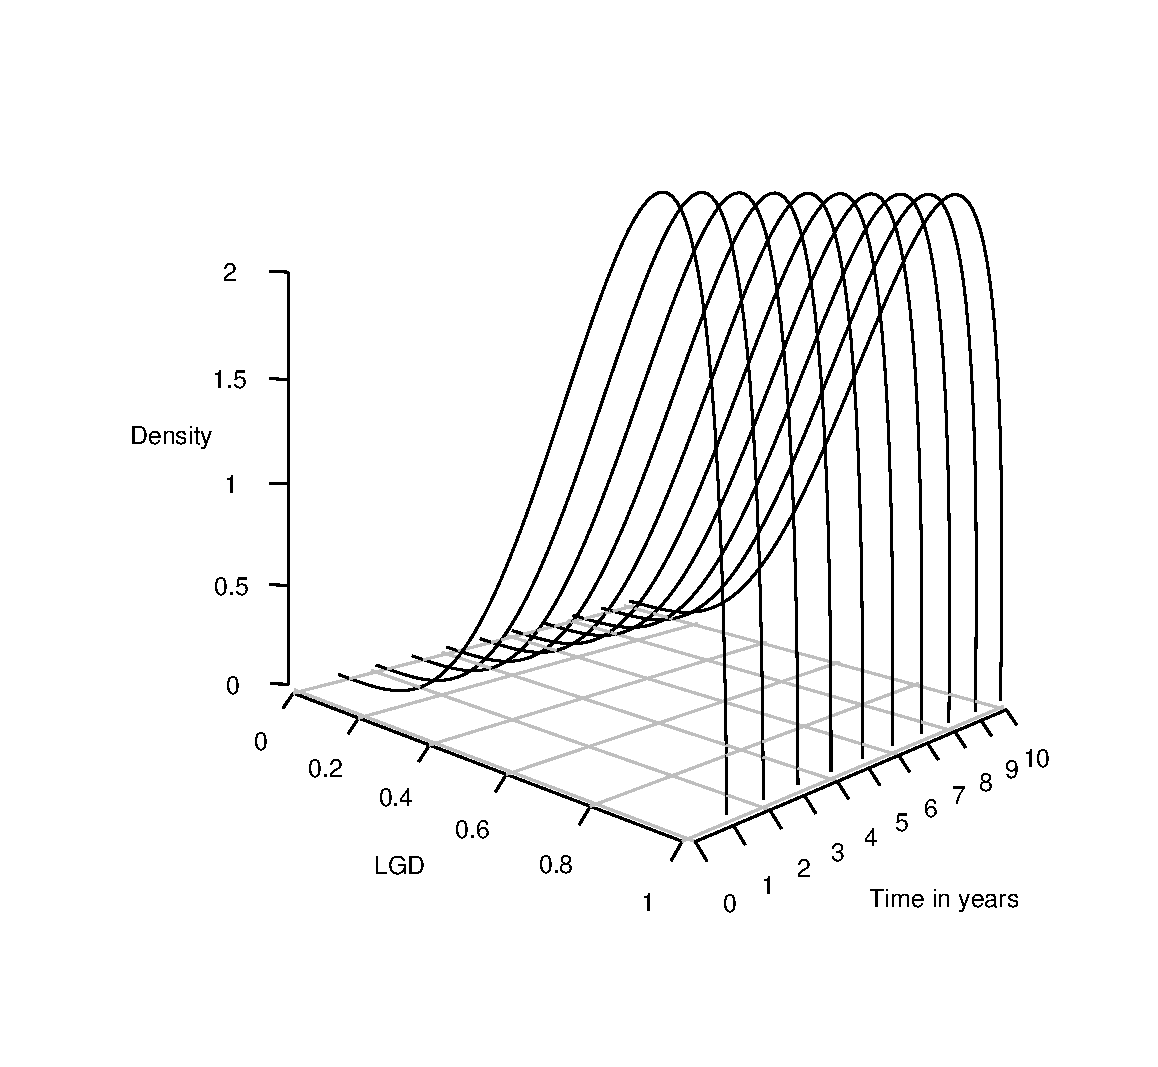
\includegraphics[width=7cm]{bond_lgd}
			\vspace{11pt}
		}
		\caption{10-years bond example}
		\label{figure:bond} 
	\end{figure}
\end{example}

\begin{comment}
\begin{example}[Bond]
	Let a 10-years fixed rate bond with an annual coupon of the
	$4\%$ issued by a company rated BB\@. The credit rating agency 
	reports, for this obligor and rating, the PD over time displayed 
	in figure~\ref{figure:bond} with a $\text{PD}(1)=1.06\%$. 
	The EAD for this asset can be obtained from its expected cashflows 
	because they are known in advance. We suppose that the bank 
	internal models indicate that in this case the LGD is a 
	$\text{Beta}(5,2)$ distribution regardless of the default time.
	Figure~\ref{figure:bond} illustrates the defined basic concepts 
	applied to this issuer and bond.
	\begin{figure}[!ht]
		\centering
		\subcaptionbox{Probability of Default}{
			\includegraphics[width=7cm]{bond_pd1}
		}
		\subcaptionbox{Probability of Default (zoom)}{
			\includegraphics[width=7cm]{bond_pd2}
		}
		\\
		\subcaptionbox{Exposure At Default}{
			\includegraphics[width=7cm]{bond_ead}
		}
		\subcaptionbox{Loss Given Default}{
			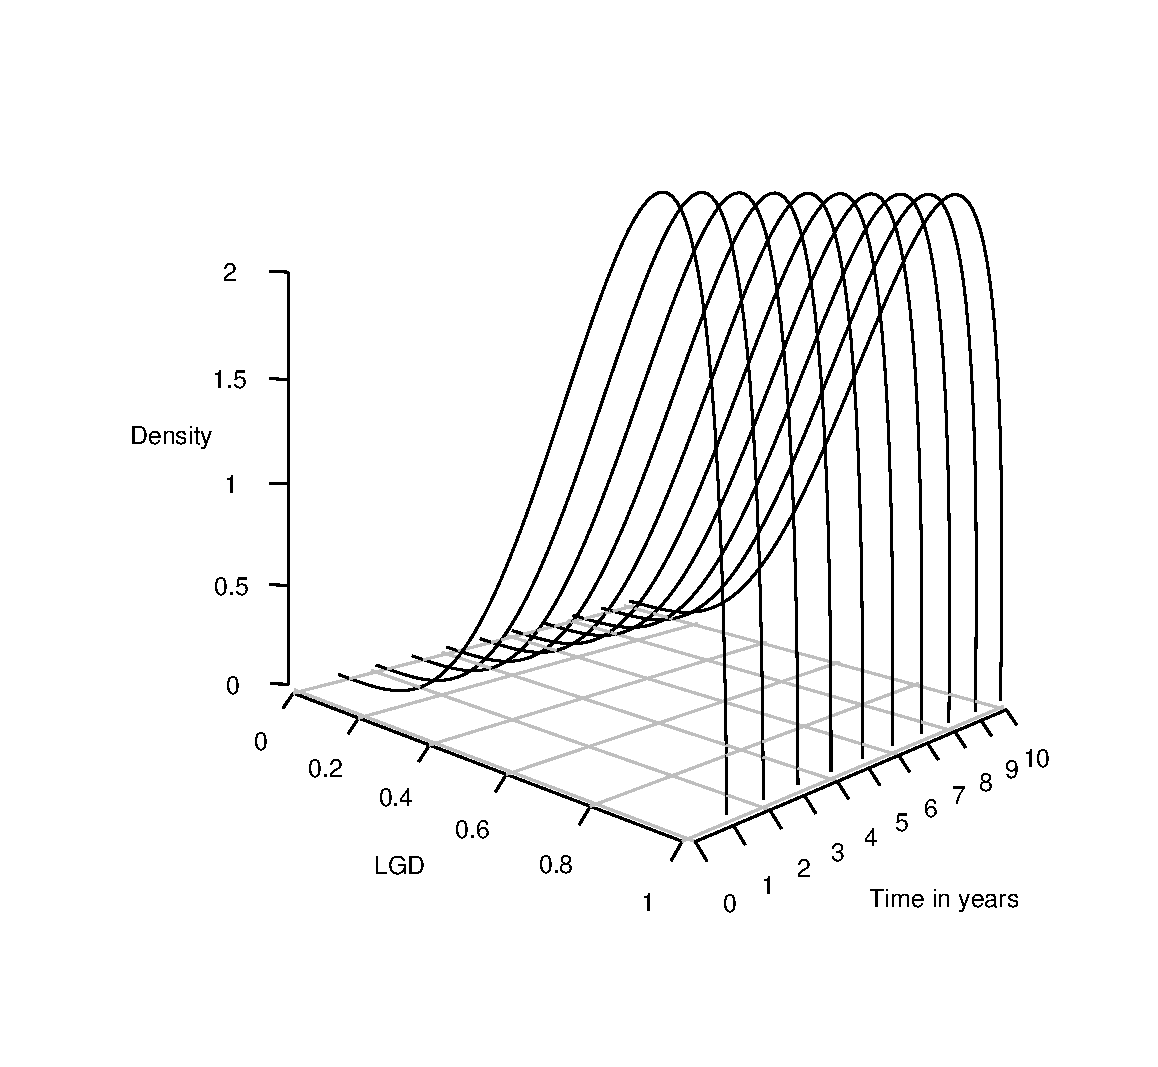
\includegraphics[width=7cm]{bond_lgd}
		}
		\caption{Basic concepts bond example}
		\label{figure:bond} 
	\end{figure}
\end{example}
\end{comment}

\begin{definition}[Portfolio Loss at time $T$]
	The Portfolio Loss at time $T$ is the cumulated losses in the time 
	range $[0,T]$ caused by obligors that defaults (fails to make 
	payments which they are obligated to do).
	\begin{displaymath}
		L_T = \left\{
		\begin{array}{c}
			\text{sum of portfolio losses in time range $[0,T]$}
		\end{array}
		\right\}
	\end{displaymath}
\end{definition}

Let a credit portfolio where the obligors default times $(T_1,\dots,T_n)$ 
is a multivariate distribution with marginals $\text{PD}_i$ and a 
t-Student copula with $\nu$ degrees of freedom and a obligors correlation
matrix $B_k(\vec{n},\vec{1},M)$. Also, each obligor $i$ has $m_i$ assets 
with known EAD and LGD\@. Then, the portfolio loss distribution at time 
horizon $t$ is:
\begin{displaymath}
	L_t = \displaystyle \sum_{i=1}^n \mathbbm{1}_{[0,t]}(T_i) \cdot 
	\left( 
	\sum_{j=1}^{m_i} \text{EAD}_j(T_i) \cdot \text{LGD}_j(T_i)
	\right)
\end{displaymath}

The portfolio loss distribution $L_t$ does not have a closed-form except 
for a few cases. One of them is the Large Homogeneous Pool (LHP).
Vasicek~\cite{vasicek:1987} derived an analytical formula for the loss 
distribution of an infinitely large portfolio. Later, Schloegl and O'Kane 
\cite{schloegl:2005} extended it to the t-Student case. The assumptions of 
these approximations are: 
\begin{inparaenum}[1)]
	\item one-factor model, 
	\item infinitely large portfolio, 
	\item equals PDs, and
	\item equals exposures
\end{inparaenum}
. These simplified models must be managed 
with care as it can cause problems~\cite{long:2012} when the assumptions 
are not satisfied.

CCruncher generates samples of the portfolio loss distribution simulating 
the obligors default times applying the corollary~\ref{cor:dts2}.

\begin{algorithm}[Portfolio losses sampling]
	\label{alg:pldmc}
	Let a multivariate default times distribution with marginals $\text{PD}_i$
	and a t-Student multi-factor model with $k$ factors, factor loadings $\vec{w}$, 
	factors correlation matrix $R$, degrees of freedom $\nu$. Then, we can 
	simulate a sample of size $T$ of the portfolio loss distribution by doing:
	\begin{enumerate}
		\item Compute the Cholesky decomposition of R, $R = L \cdot L^\intercal$
		\item For $t=1,\dots,T$ repeat the following steps
		\begin{itemize}
			\item $\text{Loss}^t = 0$
			\item Simulate $k$ independent $N(0,1)$, $\vec{z}$
			\item Simulate factors doing $\vec{z} = L \cdot \vec{z}$
			\item Simulate $v \sim \chi_{\nu}^2$
			\item For $i=1,\dots,n$ repeat the following steps
			\begin{itemize}
				\item Set $s = $ obligor factor index
				\item Set $r = $ obligor rating index
				\item Simulate $\epsilon \sim N(0,1)$
				\item Compute $x_i = \sqrt{\frac{\nu}{v}} \cdot \left( w_s \cdot z_s + \sqrt{1-w_s^2} \cdot \epsilon \right)$
				\item Compute $t_i = \text{PD}_r^{-1}\left(t_{\nu}(x_i)\right)$
				\item if $t_i \le t$ then do for each asset $l$ belonging to i-th obligor
				\begin{itemize}
					\item $\text{Loss}^t = \text{Loss}^t + \text{EAD}_l(t_i) \cdot \text{LGD}_l(t_i)$
				\end{itemize}
			\end{itemize}
		\end{itemize}
	\end{enumerate}
\end{algorithm}

\begin{example}[Large Homogeneous Pool]
	\label{ex:test04}
	Let a portfolio composed of 1000 identical obligors (with same rating 
	and sector) where every one of them owe 1\euro\ to 1 year. The common default 
	1-year probability is $p=10\%$ and the factor loading is $20\%$. This 
	problem is close to fulfill the LHP assumptions. In the Gaussian case the 
	density is~\cite[chap. 2.5]{bluhm:2002}: 
	\begin{displaymath}
		f_{p,w}(x) = 
		\frac{\sqrt{1-w^2}}{w} \cdot \exp\left( 
			\frac{\left(N^{-1}(x)\right)^2}{2} -
			\frac{\left(N^{-1}(p) - \sqrt{1-w^2} \cdot N^{-1}(x)\right)^2}{2 \cdot w^2}
		\right)
	\end{displaymath}
	where $w$ is the factor loading, $p$ is the probability to 1-year horizon, 
	and $x \in (0,1)$ represents the percentage of loss in the portfolio. 

	File \texttt{\$CCRUNCHER/samples/test04.xml} contains the CCruncher input
	file of this example. The figure~\ref{fig:test04} display the theoretical
	distribution provided by LHP approach and the approximated by CCruncher.
	Both are very similar, as expected. If we reduce the number of obligors from
	1000 to 100, then the LHP assumptions are broken and the distribution 
	provided by the LHP approach fails.
	\begin{figure}[!ht]
		\centering
		\subcaptionbox{1000 obligors}{
			\includegraphics[width=7cm]{test04-1}
		}
		\subcaptionbox{100 obligors}{
			\includegraphics[width=7cm]{test04-2}
		}
		\caption{Large Homogeneous Pool example}
		\label{fig:test04} 
	\end{figure}
\end{example}
\begin{comment}
# bash command
bin/ccruncher-cmd -w -o data/test04-1000 samples/test04-1000.xml
bin/ccruncher-cmd -w -o data/test04-100 samples/test04-100.xml
\end{comment}

\begin{example}[2 factors]
	\label{ex:test05}
	Let a portfolio composed of 1000 obligors where every obligor owe 1\euro\ to 
	1 year, this means that $\text{EAD}(t) = \mathbbm{1}_{[0,1]}(t)$, with 
	a LGD of $100\%$. There are 4 ratings \{A, B, C, D\} where D is the 
	defaulted status and the other ones have the following 1-year default 
	probability: $p_A = 5\%, p_B = 10\%, P_C = 20\%$. Factors loadings are 
	$\vec{w} = (0.4, 0.35)$ and the factors correlation is 
	$\text{Cor}(S_1,S_2) = 0.25$. The t-Student copula has $\nu=15$ degrees
	of freedom and the number of obligors by sector and rating are:

	\hspace*{1cm}
	\begin{tabular}{|c|c|c||c|c|c|}
		\hline
		\multicolumn{3}{|c||}{S1} & \multicolumn{3}{|c|}{S2} \\
		\hline
		A & B & C & A & B & C \\
		\hline
		167 & 166 & 167 & 167 & 167 & 166 \\
		\hline
	\end{tabular}
	
	% We use the proposition~\ref{prop:tmfm} to infere the correlations between
	% obligors based on its sector belonging:
	% \begin{displaymath}
		% \begin{array}{l}
			% \text{Cor}(S1,S1) = 0.4 \times 0.4 = 16\% \\
			% \text{Cor}(S1,S2) = 0.4 \times 0.35 \times 0.25 = 3.5\% \\
			% \text{Cor}(S2,S2) = 0.35 \times 0.35 = 12.25\%
		% \end{array}
	% \end{displaymath}

	File \texttt{\$CCRUNCHER/samples/test05.xml} contains the CCruncher input
	file of this example. Figure~\ref{fig:test05} display the portfolio
	loss density approximated using the random sample generated by CCruncher.
	Observe the asymmetry of the distribution. This is more pronounced when 
	$\nu$ is close to $2$, or factor loadings move away from $0$, or factor 
	correlations move away from $0$.

	It is difficult to check this example. Some authors~\cite{cespedes:2002}
	obtained quasi analytical expressions for the Gaussian two-factor model 
	with a common PD, but this is not applicable to this example (t-Student, 
	multiple PDs).
	One way to check that the result is correct consist in disaggregate the
	simulated portfolio losses by sector-rating (see section~\ref{ss:ra}) and 
	estimate the parameters $\nu, \vec{w}$, and $R$ with the first 1000 
	simulations. If the estimated values match the simulated values means 
	we have a consistent simulation and estimation algorithms. Note that in 
	this case the simulated losses can be equated to the number of defaults
	because every defaulted obligor is computed as a 1\euro\ loss.
	\begin{figure}[ht]
		\centering
		\includegraphics[width=0.98\textwidth]{test05}
		\caption{2-factors example}
		\label{fig:test05}
	\end{figure}
\end{example}

%------------------------------------------------------------------------------
% CREDIT RISK MEASUREMENT
%------------------------------------------------------------------------------
\section{Credit Risk Measurement}
\label{sec:riskm}

The portfolio credit risk is measured considering some statistics on 
the portfolio loss distribution. Figure~\ref{fig:lossdistr} illustrates 
the concepts exposed in this section.
\begin{figure}[!ht]
	\centering
	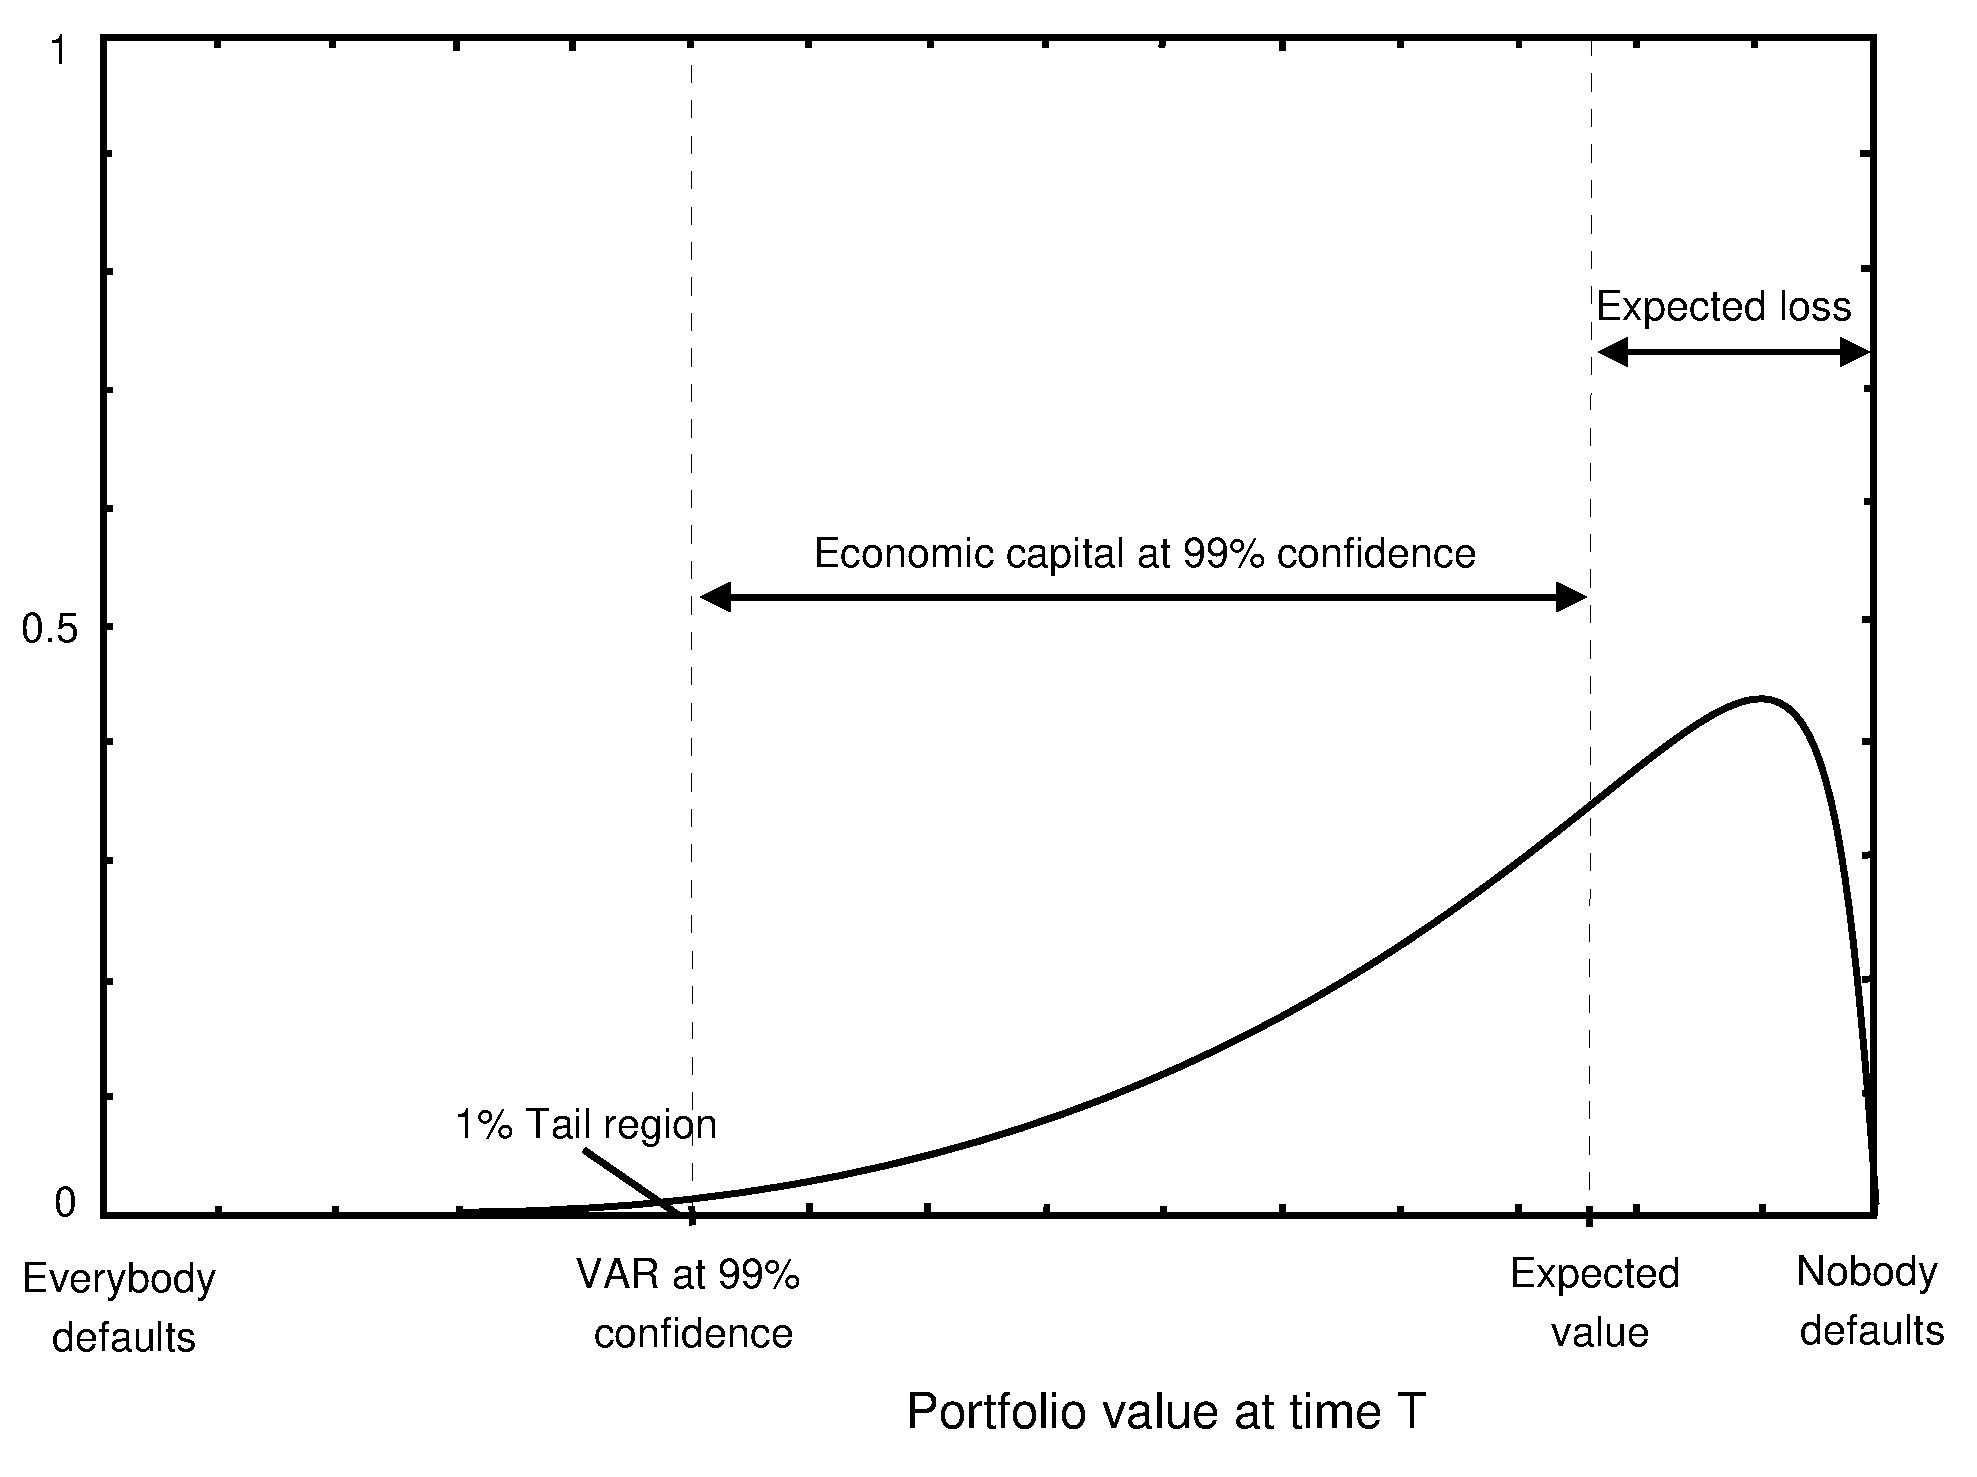
\includegraphics[width=12cm]{creditvar}
	\caption{Portfolio Loss Distribution at time $T$}
	\label{fig:lossdistr}
\end{figure}

After $N$ simulations (eg.\ $20000$, $500000$ or more) we have a list
of values $\{x_1, \ldots, x_N\}$ sampled from the portfolio loss distribution. 
We measure the portfolio credit risk computing the corresponding statistics 
and its standard errors due to sample size. Following we provide the 
definitions and formulas of the most usual credit risk measures. 
Any other risk measure can be estimated from the simulated sample and its 
standard error can be obtained using resampling methods.

When the loss values are high (eg.\ $\mathcal{O}(10^7)$) and the number of 
simulations also are high (eg.\ $\mathcal{O}(10^6)$) we can incur in a loss of 
precision when we do the sum of squares ($\mathcal{O}(10^{2 \cdot 7 + 6})$). 
The usual type used to store these values has 15--17 significant decimal 
digits precision that can be exceeded in the sum of squares. In this case it 
is recommended to use the Kahan~\cite{kahan:1965} summation algorithm.

\subsection{Expected Loss}

\begin{definition}[Expected Loss (EL)]
	The Expected Loss of a portfolio at time horizon $T$ is the 
	mean of the portfolio loss distribution.
	\begin{displaymath}
		\text{EL}(L_T) = E(L_T)
	\end{displaymath}
\end{definition}

The Expected Loss responds try to the question \enquote{what is my expected 
loss for the next year?}. It can be approximated using the following 
statistic:
\begin{displaymath}
	\text{EL} = \widehat{\mu} \pm \phi^{-1}\left(\frac{1-\alpha}{2}\right) \cdot \frac{\widehat{\sigma}}{\sqrt{N}}
	\quad \text{ being } \quad
	\left\{
	\begin{array}{l}
		\displaystyle
		\widehat{\mu} = \frac{1}{N} \sum_{i=1}^{N} x_i \\
		\\
		\displaystyle
		\widehat{\sigma} =
		\sqrt{\frac{1}{N-1} \sum_{i=1}^{N} \left( x_i - \widehat{\mu} \right)^2}
	\end{array}
	\right.
\end{displaymath}
where $\alpha$ is the error confidence level, $\phi^{-1}$ is the $N(0,1)$ 
inverse cumulative distribution function, and $\widehat{\mu}$ and 
$\widehat{\sigma}$ are the mean and standard deviation estimators.

\subsection{Value At Risk}

\begin{definition}[Value at Risk (VaR)]
	The Value At Risk of a portfolio at time horizon $T$ and 
	confidence level $\beta$ is the $\beta$-quantile of the portfolio loss 
	distribution.
	\begin{displaymath}
		\text{VaR}_\beta(L_T) = \inf\{x \in \mathbb{R} \mid F(x) \ge \beta \}
	\end{displaymath}
	where $F(x)=\Pr\{L_T \le x\}$ is the portfolio loss distribution at time $T$.
\end{definition}

The Value At Risk~\cite{var:jorion} is the most commonly 
used risk measure to respond the question \enquote{how much could I lose in a 
really bad year?}. It can be approximated using the following statistic:
\begin{displaymath}
	\begin{array}{lcl}
		\textrm{VaR}_{\beta} = \widehat{q_{\beta}} \pm \phi^{-1}\left(\frac{1-\alpha}{2}\right) \cdot \textrm{stderr}(q_{\beta})
		& \text{ being } &
		\left\{
		\begin{array}{l}
			\displaystyle
			\frac{k}{N} \leq \beta < \frac{k+1}{N} \\
			\\
			\displaystyle
			\widehat{q_{\beta}} = x_{k:N} \\
		\end{array}
		\right.
		\\
		& &
		\\
		\textrm{stderr}(q_{\beta}) = \sqrt{C_2 - C_1^2}
		& \text{ being } &
		\left\{
		\begin{array}{rcl}
			M   & = & [N \beta + 0.5]  \\
			a   & = & M - 1            \\
			b   & = & N - M            \\
			W_i & = & B(a,b,\frac{i+1}{N}) - B(a,b,\frac{i}{N}) \\
			C_k & = & \sum_{i=1}^{N} W_i \cdot x_i^k \\
		\end{array}
		\right.
		\\
	\end{array}
\end{displaymath}
where $\alpha$ is the error confidence level, $\phi^{-1}$ is the $N(0,1)$ 
inverse cumulative distribution function, $\widehat{q_{\beta}}$ is the 
quantile estimator, $x_{k:N}$ is the $k$-th element of ascendant-sorted 
values, $\textrm{stderr}(q_{\beta})$ is the estimation of the standard 
error using the Maritz-Jarret method described in~\cite{quant:algor},
$[x]$ is the integer part of $x$, and $B(a,b,x)$ is the regularized 
incomplete beta function.

\subsection{Expected Shortfall}

\begin{definition}[Expected Shortfall (ES)]
	The Expected Shortfall of a portfolio at time horizon $T$ and 
	confidence level $\beta$ is the average of the worst $\beta\%$ losses.
	\begin{displaymath}
		\text{ES}_\beta(L_T) = \text{E}(L_t \mid L_t \ge \text{VaR}_\beta(L_T))
	\end{displaymath}
\end{definition}

VaR is not a distance because it does not fulfill the sub-additive property 
\cite{var:varbad}, $\text{VaR}(A+B) \nleq \text{VaR}(A)+\text{VaR}(B)$. 
Similar to VaR, Expected Shortfall is a consistent risk measure 
\cite{var:eshortfall}. We note as
$\{y_1, \ldots, y_K\} = \{x_i \mid x_i \ge \text{VaR}_{\beta} \}_{i=1,\dots,N}$ 
the simulated portfolio losses that are bigger than $\text{VaR}_{\beta}$.
\begin{displaymath}
	\text{ES}_{\beta} = \widehat{\mu} \pm \phi^{-1}\left(\frac{1-\alpha}{2}\right) \cdot \frac{\widehat{\sigma}}{\sqrt{K}}
	\quad \text{ being } \quad
	\left\{
	\begin{array}{l}
		\displaystyle
		\widehat{\mu} = \frac{1}{K} \sum_{i=1}^{K} y_i \\
		\\
		\displaystyle
		\widehat{\sigma} =
		\sqrt{\frac{1}{K-1} \sum_{i=1}^{K} \left( y_i - \widehat{\mu} \right)^2}
	\end{array}
	\right.
\end{displaymath}
where $\alpha$ is the error confidence level, $\phi^{-1}$ is the $N(0,1)$ 
inverse cumulative distribution function, and $\widehat{\mu}$ and 
$\widehat{\sigma}$ are the mean and standard deviation estimators.
Honestly, this estimator is not the best one because it assumes that
the estimated $\text{VaR}_{\beta}$ value is the right one. Despite this, 
if the sample size is high enough then the estimated value is good enough.

%------------------------------------------------------------------------------
% SIMULATION INTERNALS
%------------------------------------------------------------------------------
\section{Simulation internals}

\textbf{PD functions approximation}. CCruncher allows defining the PDs
functions using the transition matrix or defining explicitly the values
at some fixed points. When the PDs are defined using the transition matrix 
CCruncher uses the proposition~\ref{prop:pdftm} to derive the PDs values 
for each month and intermediate values are interpolated using cubic splines. 
When the PDs values are defined explicitly at fixed time values, then 
intermediate values are also interpolated using cubic splines but if the 
resulting function is not strictly increasing, we use linear splines.

\textbf{EAD and LGD interpolation}. Given an asset, CCruncher knows its EAD 
and LGD values at fixed times $\{t_1,\dots,t_n\}$ provided by user. When 
we evaluate these functions in a time value distinct than those provided we 
use the following piecewise constant interpolation:
\begin{displaymath}
	F(t) = F(t_k) \quad \text{where} \quad t_{k-1} < t \le t_{k}
\end{displaymath}
\textbf{Function composition}. In order to speed-up the evaluation of the
function $t=\text{PD}_r^{-1}(t_{\nu}(x))$ used in the default times simulation
we approximate it using linear splines at a selected set of days $\mathbb{S}$. 
Let $\{t_1,\dots,t_n\}$ the days where $\text{PD}_r$ has known values (not 
interpolated), and let $t=P(x)$ the function $t=\text{PD}_r^{-1}(t_{\nu}(x))$ 
linearly interpolated using the current points of set $\mathbb{S}$. 
Then, CCruncher determines the set of days $\mathbb{S}$ using the following 
procedure:
\begin{itemize}
	\item Add the first day of the simulation time range to $\mathbb{S}$, $d_1$.
	\item Add the last day of the simulation time range to $\mathbb{S}$, $d_T$.
	\item Repeat until $\displaystyle \max_{d_1 \le d \le d_T}\left|d - P(t_{\nu}^{-1}(\text{PD}_r(d)))\right| < 1$ hour
	\begin{itemize}
		\item Let $d$ the day where maximum error is achieved
		\item Let $t_i \le d \le t_{i+1}$ the nearest days where $\text{PD}_r$ is defined
		\item If $t_i$ is not contained in $S$, add $t_i$ to $\mathbb{S}$
		\item Else if $t_{i+1}$ is not contained in $\mathbb{S}$, add $t_{i+1}$
		\item Else add $d$ to $\mathbb{S}$
	\end{itemize}
\end{itemize}

\textbf{Interest rate}. CCruncher allows to consider the Net Present Value 
of the simulated losses. This is computed using an interest rate curve 
defined at fixed times and interpolated using linear or cubic splines 
(selected by user). Allowed methods are simple interest, compound interest 
and continuous interest. The formulas used to compute the present value are:
\begin{center}
	\begin{tabular}{ccccc}
		$V_0 = \frac{V_t}{1+r \cdot \Delta t}$ & $\qquad$ &
		$V_0 = \frac{V_t}{(1+r)^{\Delta t}}$ & $\qquad$ &
		$V_0 = \frac{V_t}{\exp(r \cdot \Delta t)}$ \\
		(Simple) & $\qquad$ & (Compound) & $\qquad$ & (Continuous)
	\end{tabular}
\end{center}
where $V_t$ is the value at time $t$, and $r$ is the interest rate given 
by the interest curve at time $t$. This option does not make much sense
if your EAD are the sum of cashflows at distinct dates. If you want to work 
with net values we recommend that you put the present value of the EADs and 
set the interest rate curve to $0$.

\textbf{Risk aggregation}. 
\label{ss:ra}
CCruncher simulates the whole portfolio loss at time $T$. It also allows (in 
the same execution) the simulation of sub-portfolios losses. The name to refer
a sub-portfolio is \emph{segment}. A segmentation is the disjoint union of some 
segments that constitutes the whole portfolio so that an asset belongs to only 
one segment of a given segmentation. By example, we can define a segmentation
of assets where the segments are bonds, loans, leases, etc. Each asset
belongs to only one segment. When an obligor defaults, the loss of its assets
are aggregated to the whole portfolio loss, and the loss of each of its assets
is aggregated to the corresponding segment. CCruncher allows defining and 
managing multiple segmentations simultaneously. The segmentations can be 
composed of obligors or assets. In the first case, the obligor loss is 
aggregated to segment loss when the obligor defaults. In the second case, the 
asset losses are aggregated to segments losses when the obligor defaults.

\textbf{Parallel computing}. 
CCruncher parallelize the portfolio loss sampling spawning multiple simulation
threads, each of them with its own Mersenne twister Random Number Generator 
seeded with consecutive values. When the number of obligors is high, data 
don't fit in the cache memory L1 and L2. The memory transfer is a time expensive
operation that must be minimized. To achieve this, CCruncher simule each 
obligor \emph{blocksize} times (each of them with the corresponding $\nu$ and 
$\vec{z}$) before moving to the next obligor. This strategy can be considered 
to implement CCruncher parallelization in CUDA-like architectures.

%------------------------------------------------------------------------------
% VARIANCE REDUCTION
%------------------------------------------------------------------------------
\section{Variance Reduction}

Monte Carlo method consists on sampling a distribution and averages these
values to approximate the mean of this distribution. The main drawback 
of this method is the low rate of convergence that is of order $1/\sqrt{N}$.
Variance reduction methods are procedures used to increase the precision 
of the estimates of the Monte Carlo method. The main ones are: common random 
numbers, antithetic variates, control variates, importance sampling and 
stratified sampling.

CCruncher generate random samples from the portfolio loss distribution.
This sample is used to estimate the risk measures (eg.\ VaR) using the 
statistics described in section~\ref{sec:riskm} or any other required 
by the analyst. Anyone of these measures, considered one by one, can be 
formulated as a Monte Carlo problem and we apply some variance 
reduction techniques, but not simultaneously. Expected Loss is the only 
statistic that can be formulated directly as a Monte Carlo formulation 
using the CCruncher simulated values.

For this reason the variance reduction techniques used in CCruncher 
don't aims the increase of precision, but improve the overall result in 
some manner. The applied variance reduction procedures implemented in
CCruncher are the following.

\subsection{Antithetic variates}
We are estimating $E(g(X))$ using the Monte 
Carlo method. Let $Y_1$ and $Y_2$ random variables with the same distribution
$g(X)$. This means that $E(g(X)) = E(Y_1) = E(Y_2) = E(\frac{Y_1+Y_2}{2})$ and
$\text{Var}\left(\frac{Y_1+Y_2}{2}\right) = 
\frac{\text{Var}(Y_1)+\text{Cov}(Y_1,Y_2)}{2}$.
If $Y_1$ and $Y_2$ are negatively correlated then the variance of $N$ 
simulated values from $\frac{Y_1+Y_2}{2}$ is smaller than the variance 
of $2{\times}N$ simulated values from $Y_1$ or $Y_2$.

In CCruncher we use the fact that the multivariate t-Student distribution 
$X$ is symmetrical, that is, $(x_1,\dots,x_n)$ is equiprobable to 
$(-x_1,\dots,-x_n)$. The random sampling of the portfolio loss 
distribution is performed doing $g(X)$ where $X$ is a multivariate t-Student
distribution and $g(x) = \text{PD}^{-1}(t_{\nu}(x))$, thus, $g(X)$ and $g(-X)$ 
are equiprobables. The only estimator that reduces the variance for this cause 
is the Expected Loss. But rather than reducing the variance we are interested 
in the reusing of the simulated random numbers to increase the simulation 
speed. Please note, when there are stochastic EADs or LGDs and we use the
antithetic method to sample the default times, we use a distinct random values
of the EADs and LGDs for each variate.

\begin{lstlisting}[language=R, label=sc:antithetic, caption=Antithetic example (R script)]

 f <- function(x) { 1/(1+x) }
 result = matrix(nrow=4, ncol=3)
 colnames(result) = c("N", "Mean", "Var")
 rownames(result) = 1:4

 rownames(result)[1] = "Exact";
 result[1,1] = 0
 result[1,2] = integrate(f, lower=0, upper=1)$value
 result[1,3] = 0

 u = runif(10000)
 rownames(result)[2] = "Monte Carlo";
 result[2,1] = length(u)
 result[2,2] = mean(f(u))
 result[2,3] = var(f(u))

 u = runif(5000)
 rownames(result)[3] = "Antithetic";
 result[3,1] = length(u)
 result[3,2] = mean((f(u)+f(1-u))/2)
 result[3,3] = var((f(u)+f(1-u))/2)

 u = runif(5000)
 u = c(u, 1-u)
 rownames(result)[4] = "CCruncher";
 result[4,1] = length(u)
 result[4,2] = mean(f(u))
 result[4,3] = var(f(u))

\end{lstlisting}
\hspace*{1cm}
\begin{tabular}{l|c|c|c|}
	\cline{2-4}
	& N & Mean & Var \\
	\hline
	\multicolumn{1}{|l|}{Exact} & 0 & 0.693147 & 0.000000 \\
	\hline
	\multicolumn{1}{|l|}{Monte Carlo} & 10000 & 0.695685 & 0.019624 \\
	\hline
	\multicolumn{1}{|l|}{Antithetic} & 5000 & 0.693404 & 0.000593 \\
	\hline
	\multicolumn{1}{|l|}{CCruncher} & 10000 & 0.693099 & 0.019508 \\
	\hline
\end{tabular}
\vspace{11pt}

\subsection{Latin Hypercube Sampling (LHS)}
This variance reduction technique 
belongs to the stratified sampling family. It consists in divide the total 
probability range ($100\%$) in $N$ equispaced segments. Then we create a 
sample of size $N$ picking a random value from each segment using a uniform 
distribution and applying the inverse transform sampling. Finally we shuffle 
the sample to obtain the desired distribution random values. When we have 
two independent random variables, we repeat the above procedure for each of 
them obtaining the Latin Square effect: the generated random points are in
a reticle where each row and column has only one point. The procedure for
three or more independent variables is exactly the same and its named Latin 
Hypercube Sampling~\cite{jorgensen:1998,glasserman:1997}.

When the random variables are dependent the previous schema doesn't work 
and it is reformulated recurring to copulas and the rank statistic 
\cite{wolfgang:2008}. In this case the number of bins has impact in the 
quality of the generated values, the bigger the better.

In CCruncher, the random variables that can be sampled using the LHS 
technique are the degrees of freedom, $\nu$, and the factors, $\vec{z}$. 
The aim is to ensure a uniform scanning of these variables so that the
extreme cases are represented.

\begin{lstlisting}[language=R, label=sc:lhs, caption=Latin Hypercube Sampling example (R script)]

 rlhs <- function(nblocks, icdf, ...) 
 {
   ret = rep(NA,nblocks)
   for(i in 1:nblocks) {
     u = runif(1, min=(i-1)/nblocks, max=i/nblocks)
     ret[i] = icdf(u, ...)
   }
   ret = sample(ret)
   return(ret)
 }

 x1 = rnorm(100, mean=0, sd=1)
 cdf1 = ecdf(x1)
 plot(cdf1, verticals=TRUE, pch=26, ylab="prob", main="");
 
 x2 = rlhs(100, qnorm, mean=0, sd=1)
 cdf2 = ecdf(x2)
 plot(cdf2, verticals=TRUE, pch=26, ylab="prob", main="");
 
\end{lstlisting}
\begin{figure}[!ht]
	\centering
	\subcaptionbox{Empirical cdf (without lhs)}{
		\includegraphics[width=7cm]{lhs1}
	}
	\subcaptionbox{Empirical cdf (using lhs)}{
		\includegraphics[width=7cm]{lhs2}
	}
	\caption{Latin Hypercube Sampling example (1-dim)}
	\label{fig:lhs} 
\end{figure}

%------------------------------------------------------------------------------
% PARAMETERS UNCERTAINTY
%------------------------------------------------------------------------------
\section{Parameters Uncertainty}

The estimation of dependence parameters (degrees of freedom $\nu$, factor
loadings $\vec{w}$, and factors correlation $R$) has an uncertainty that 
cannot be ignored~\cite{tarashev:2010,gossl:2005}. The example~\ref{ex:calib} 
illustrates this phenomenon and its magnitude (see the 20 observations case).

The CCruncher framework encourages incorporating the parameter uncertainty 
in the credit risk valuation. This means that some credit risk measures
(eg.\ $\text{VaR}_{99\%}$, $\text{ES}_{99\%}$) are therefore regarded as 
distributions instead of precise values. As example, in the case of the Value 
at Risk, we consider it as a distribution $\text{VaR}_{99\%}(\nu,\vec{w},R)$ 
that depends on multivariate random variables $\nu, \vec{w}$ and $R$.

Note that the EL measure is not affected by the uncertainty of dependence 
parameters because the expectation satisfies $E(X+Y)=E(X)+E(Y)$ even if $X$ 
is not statistically independent of $Y$.

The solution recommended by CCruncher to determine the distribution of a
credit risk measure is the obvious. It is based in the same procedure 
used to determine the distribution of the portfolio loss, or the distribution 
of the parameters: the random sampling of the risk measure distribution. 

On one hand we are able to measure the credit risk of a portfolio presupposing 
that dependence parameters are fixed values. This is done sampling the portfolio
loss (algorithm~\ref{alg:pldmc}) and approximating the credit risk indicator
using the appropriate statistic (see section~\ref{sec:riskm}). The risk 
measure obtained by this procedure consist of an approximated value an
a standard error that allows to define a confidence interval fixed a 
confidence level (eg.\ 95\%).

On the other hand we have a procedure (see proposition~\ref{prop:pemh}) that 
generate random samples from the multivariate parameters distribution.
These samples can be filtered in order to obtain a sample of independent
parameters values. We note this sample of the parameters distribution as
$\{\nu^t, \vec{z}^t, R^t\}_{t=1,\dots,N}$.

\begin{algorithm}[Credit risk measure distribution]
	\label{alg:crmd}
	Let a portfolio (ratings, sectors, PDs, EADs, LGDs) and the numbers 
	of defaults observed by sector-rating in the previous years. We can
	determine the distribution of a credit risk measure 
	(eg.\ $\text{VaR}_{99\%}$) doing:
	\begin{enumerate}
		\item Obtain an ergodic sample of the parameters applying the
		Metropolis-Hastings algorithm (see proposition~\ref{prop:pemh}).
		\item Remove the first iterations (burnin period) and determine
		the length $B$ at which the autocorrelation is $0$.
		\item Let $\{\nu^t, \vec{z}^t, R^t\}_{t=1,\dots,N}$ the subsample
		of the parameters distribution composed by the indexes multiples 
		of $B$.
		\item For each simulated parameters simule the portfolio loss 
		distribution using the algorithm~\ref{alg:pldmc}.
		\item For each simulated portfolio loss distribution compute its 
		risk measure using the statistic described in~\ref{sec:riskm}:
		$\{\text{VaR}_{99\%}^t(\nu^t,\vec{w}^t,R^t)\}_{t=1,\dots,N}$.
	\end{enumerate}
\end{algorithm}

\begin{example}[Credit risk considering parameters uncertainty]
	\label{ex:paramu}
	We use the same scenario that is described in the example~\ref{ex:test05} 
	and that correspond to CCruncher input file 
	\texttt{\$CCRUNCHER/samples/test05.xml}. 
	We generate 20 observations using the algorithm~\ref{alg:snod}. In the real 
	world these observations are extracted from the historical records. 
	In this example we apply the algorithm~\ref{alg:crmd} to estimate the 
	$\text{ES}_{99\%}$ distribution taking into account the parameters 
	uncertainty. 

	The first step consists in the generation of a sample of the parameters 
	distribution using the Metropolis-Hastings algorithm. We perform 1000000
	of iterations. Figure~\ref{fig:paramu1} displays the marginals of this 
	distribution.
	\begin{figure}[!ht]
		\centering
		\includegraphics[width=0.98\textwidth]{paramu-1}
		\caption{Parameters simulation using M-H}
		\label{fig:paramu1}
	\end{figure}
	
	The second step consist in determine the thin interval using the 
	autocorrelation functions. Figure~\ref{fig:paramu2} shows the ACF for 
	each parameter. A thin interval of 3000 is sufficient in this example. 
	\begin{figure}[ht]
		\centering
		\includegraphics[width=0.98\textwidth]{paramu-2}
		\caption{Autocorrelation function of simulated parameters}
		\label{fig:paramu2}
	\end{figure}
	
	The third step consist in pruning the parameters sample preserving 
	only the simulated values whose index is a multiple of 3000. 
	Table~\ref{tab:paramu3} displays part of the simulated values.
	\begin{table}[!ht]
		\centering
		\begin{tabular}{cc|c|c|c|c|}
			\cline{1-1} \cline{3-6}
			\multicolumn{1}{|c|}{It} & & $\nu$ & $w_1$ & $w_2$ & $R_{12}$ \\
			\cline{1-1} \cline{3-6}
			\multicolumn{1}{|c|}{1} & & 12.54 & 0.29 & 0.48 & 0.21 \\
			\cline{1-1} \cline{3-6}
			\multicolumn{1}{|c|}{2} & & 10.77 & 0.28 & 0.32 & -0.28 \\
			\cline{1-1} \cline{3-6}
			\multicolumn{1}{|c|}{\vdots} & & \vdots & \vdots & \vdots & \vdots \\
			\cline{1-1} \cline{3-6}
			\multicolumn{1}{|c|}{300} & & 10.06 & 0.33 & 0.36 & 0.02 \\
			\cline{1-1} \cline{3-6}
		\end{tabular}
		\caption{Simulated parameters}
		\label{tab:paramu3}
	\end{table}

	The fourth step is the simulation of the portfolio loss distribution
	for each simulated parameters. This is a very intensive computation.
	CCruncher provides a command line incarnation and a macro expansion in
	the input file that can help to do this step. If you have a cluster, a 
	cloud or grid you can consider to execute multiple task in parallel using 
	a framework like 
	MakeFlow\footnote{\url{http://www3.nd.edu/~ccl/software/makeflow/}} 
	or similar. Listing~\ref{sc:paramu4} displays a very simple batch
	script to execute sequentally the required simulations.
	\begin{lstlisting}[language=bash, label={sc:paramu4}, 
	caption={Execution of multiple CCrunchers (bash script)}]
 
 mkdir data/MH001;
 bin/ccruncher-cmd -o data/MH001 -DNU=12.54 -DW1=0.29 \
     -DW2=0.48 -DR12=0.21 samples/test05.xml; 
 
 mkdir data/MH002; 
 bin/ccruncher-cmd -o data/MH002 -DNU=10.77 -DW1=0.28 \
     -DW2=0.32 -DR12=-0.28 samples/test05.xml; 

 ...

 mkdir data/MH300; 
 bin/ccruncher-cmd -o data/MH300 -DNU=10.06 -DW1=0.33 \
     -DW2=0.36 -DR12=0.02 samples/test05.xml; 
 
	\end{lstlisting}

	Finally, the fifth step is the computation of the risk statistic
	for each portfolio loss distribution. The density of the $\text{ES}_{99\%}$ 
	can be approximated using the estimated density. Listing~\ref{sc:paramu5}
	provides an R script to do this task. 
	\begin{lstlisting}[language=R, label={sc:paramu5}, 
	caption={$ES_{99\%}$ distribution (R script)}]

 getRisk <- function(dir)
 {
   filename = paste(dir, "/portfolio.csv", sep="")
   data <- read.csv(filename, header=T)
   X = sort(data[,1])
   n = length(X)
   Y = X[as.integer(n*0.99):n]
   ES99 = mean(Y)
   sde = sqrt(var(Y)/length(Y))
   return(c(ES99,sde))
 }

 dirs = dir("data", pattern="MH[[:digit:]{3}]*", full.names=TRUE)
 values = matrix(ncol=2,nrow=length(dirs))
 colnames(values) = c("ES99", "stderr")
 for(i in 1:length(dirs)) {
   values[i,] = getRisk(dirs[i])
 }
 
 plot(density(values[,1]))
 
	\end{lstlisting}
	
	The exact value of the $\text{ES}_{99\%}$ assuming that parameters 
	are fixed and known is $\approx 385$\ \euro. If we don't assume that 
	parameters are known and we infer it from 20 observations of the
	numbers of defaults, then we obtain the distribution displayed in
	figure~\ref{fig:paramu5}. This distribution is highly conditioned by
	the 20 observations. In this example, the exact value is located in the
	bottom of the statistics values, but other 20 simulated values can 
	draw a density where the exact value is the upper part of the estimated 
	density. The key point is to dispose a distribution indicating the 
	feasible values that can take the risk measure $\text{ES}_{99\%}$.
	In this example it's not crazy to consider that $\text{ES}_{99\%} < 450$.
	\begin{figure}[!ht]
		\centering
		\includegraphics[width=0.98\textwidth]{paramu-5}
		\caption{$\text{ES}_{99\%}$ distribution}
		\label{fig:paramu5}
	\end{figure}
\end{example}
\begin{comment}
# R script to simulate values
source("/home/gerard/projects/ccbinf/bin/ccbinf.R")
p = c(0.05, 0.1, 0.2)
w = c(0.4, 0.35)
D = matrix(nrow=2, ncol=3, data=c(167, 167, 166, 167, 167, 166))
R = matrix(ncol=2, nrow=2, data=c(1.0,0.25,0.25,1.0))
nu = 15
rcount = ccruncher.rcount(20, p, D, w, R, nu)
export(rcount, "paramu.txt")

# bash commands
/home/gerard/projects/ccbinf/build/ccbinf -r 1000 -n 1000000 paramu.txt
\end{comment}


%==============================================================================
% APPENDICES
%==============================================================================
\appendix
\chapterimage{chapter_head_1.pdf}
\chapter{Appendices}

%------------------------------------------------------------------------------
% COPULA BASICS
%------------------------------------------------------------------------------
\section{Copula Basics}
\label{ap:copula_basics}

\begin{wrapfigure}{r}{0.5\textwidth}
	\vspace{-25pt}
	\begin{center}
		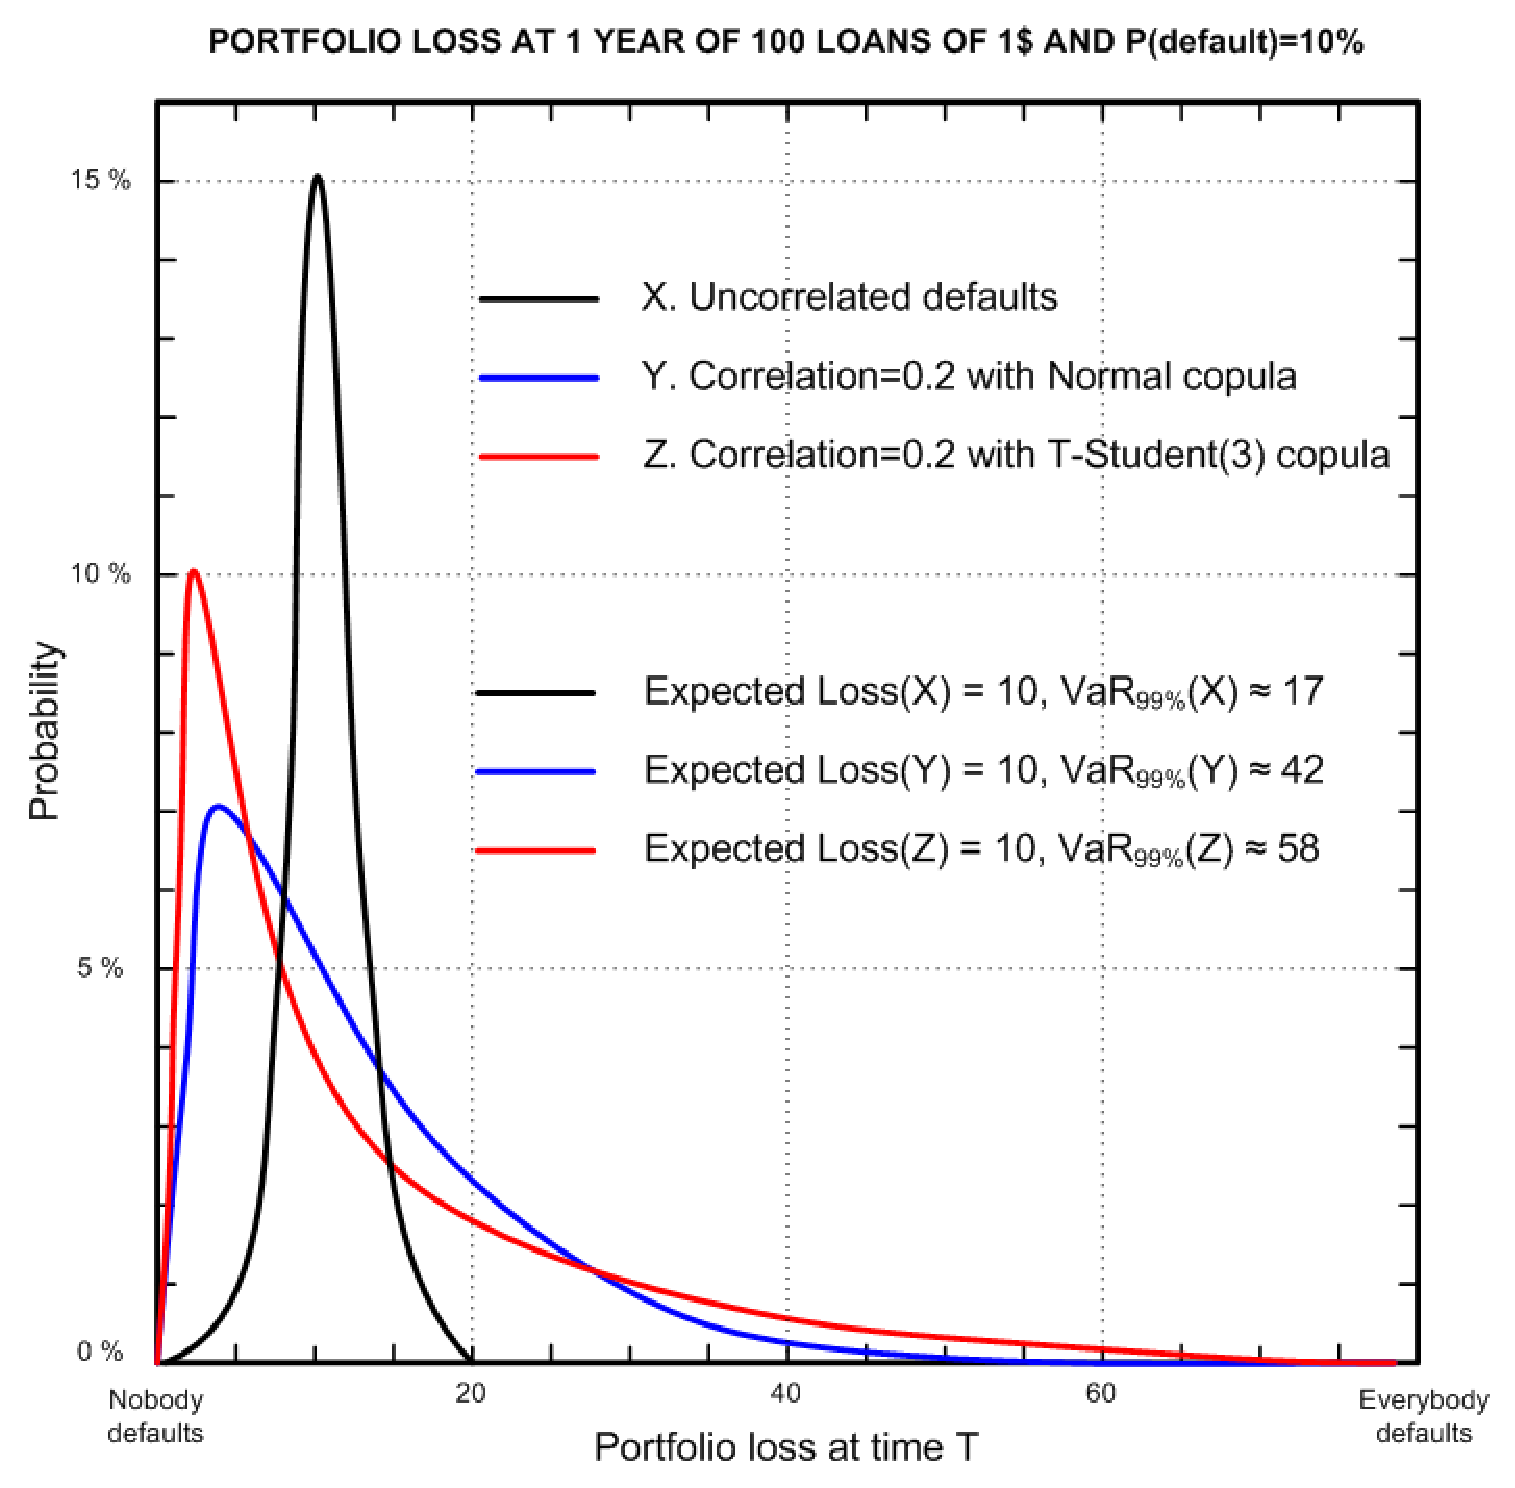
\includegraphics[width=0.48\textwidth]{ercim78}
	\end{center}
	\vspace{-10pt}
	\caption{Dependence structure impact}
	\vspace{-10pt}
	\label{fig:copula_impact}
\end{wrapfigure}
It is common to use correlation as a measure of dependency between random 
variables. In most cases, this measure does not fully reflect the structure 
of dependence between them. Figure~\ref{fig:copula_impact} displays two
cases with the same mean, marginals and correlations but a distinct risk
profile because its underlying  dependence structure is distinct (Gaussian 
copula vs.\ t-Student(3) copula). The mathematical concept that does reflect 
the structure of dependence between random variables, however, is the copula, 
which we define below. The world of copulas is vast and very interesting. 
See~\cite[chap. 5]{mcneil:2005} for a pleasant and detailed introduction to 
copulas.

\begin{definition}[Copula]
	A copula function, $C$, is a multivariate distribution defined on the 
	unit hypercube $[0,1]^d$ with standard uniform marginals. 
	More precisely,
	\begin{displaymath}
		C(u_1, \dots, u_d) = \Pr\{U_1 \le u_1, \dots, U_d \le u_d\}
	\end{displaymath}
	where $U_i \sim \text{Uniform}(0,1) \text{ for } i = 1,\dots, d$.
\end{definition}

Sklar's theorem~\cite{sklar:1959} states that any multivariate 
distribution with continuous marginals can be decomposed into the marginals and 
a copula that reflects the structure of dependence between them. Later, we will 
use this statement to define and simulate the t-Student copula.

\begin{theorem}[Sklar's theorem]
	\label{thm:sklar}
	Let $F$ be an $d$-dimensional distribution function with margins $F_1,\dots,F_d$.
	Then there exists an $d$-copula $C$ such that for all $x \in \mathbb{R}^d$,
	\begin{displaymath}
		F(x_1,\dots,x_d) = C(F_1(x_1),\dots,F_d(x_d))
	\end{displaymath}
	If $F_1,\dots,F_d$ are all continuous, the $C$ is unique; otherwise $C$ is uniquely
	determined on $\text{Ran}F_1 \times \cdots \times \text{Ran}F_d$.
	Conversely, if $C$ is an $d$-copula and $F_1,\dots,F_d$ are distributions functions,
	then the function $F$ defined above is an $d$-dimensional distribution function
	with margins $F_1,\dots,F_d$.
\end{theorem}

\begin{corollary}[Copula of a multivariate distribution]
	\label{cor:cop1}
	Let $X=(X_1, \dots, X_d)$ a random vector with a multivariate 
	distribution $F$ and continuous marginals $F_1, \dots, F_n$. 
	Then its copula is:
	\begin{displaymath}
		C(u_1,\dots,u_n) = F(F_1^{-1}(u_1), \dots, F_n^{-1}(u_n))
	\end{displaymath}
\end{corollary}
%\begin{proof}
%This is a direct application of Sklar's theorem:
%\begin{displaymath}
%C(F_1(x_1), \dots, F_d(x_d)) = 
%F(F_1^{-1}(F_1(x_1)), \dots, F_d^{-1}(F_d(x_d))) = 
%F(x_1, \dots, x_d)
%\end{displaymath}
%\end{proof}

\begin{corollary}[Copula simulation]
	\label{cor:cop2}
	Let $X=(X_1, \dots, X_d)$ a random vector with a multivariate 
	distribution $F$ and continuous marginals $F_1, \dots, F_n$.
	If we have a procedure to simulate $X$ then we can simulate 
	its copula $C$ using:
	\begin{displaymath}
		(U_1, \dots, U_d) = (F_1(X_1), \dots, F_d(X_d))
	\end{displaymath}
\end{corollary}

\begin{corollary}[Multivariate distribution simulation]
	\label{cor:cop3}
	Let $X=(X_1, \dots, X_d)$ a random vector with a copula $C$
	and continuous marginals $F_1, \dots, F_n$. If we have a
	procedure to simulate $C$ then we can simulate $X$ using:
	\begin{displaymath}
		(X_1, \dots, X_d) = (F_1^{-1}(U_1), \dots, F_d^{-1}(U_d))
	\end{displaymath}
	where $U_i$ are the copula components.
\end{corollary}

%------------------------------------------------------------------------------
% MULTIVARIATE t-STUDENT DISTRIBUTION
%------------------------------------------------------------------------------
\section{Multivariate t-Student Distribution}
\label{ap:mtsd}

\begin{definition}[Multivariate t-Student distribution]
	The $d$-dimensional random vector $X=(X_1,\dots,X_d)$ is said to have a 
	(non-singular) multivariate t-Student distribution with $\nu$ degrees of freedom, 
	mean vector $\mu$ and positive-definite dispersion or scatter matrix $\Sigma$, 
	denoted $t \sim t_d(\nu,\mu,\Sigma)$, if its density is given by
	\begin{displaymath}
		f(x)=\frac{\Gamma\left(\frac{\nu+d}{2}\right)}{\Gamma\left(\frac{\nu}{2}\right)\sqrt{(\pi \nu)^d |\Sigma|}}
		\left(
		1+ \frac{(x-\mu)^\top\Sigma^{-1}(x-\mu)}{\nu}
		\right)^{-\frac{\nu+d}{2}}
	\end{displaymath}
	\noindent where $\Gamma$ is the gamma function, and $|\Sigma|$ is the 
	determinant of the matrix.
\end{definition}

\begin{proposition}[Gaussian as limit of the t-Student]
	The t-Student distribution converges to a Gaussian distribution 
	when $\nu$ tend to $\infty$.
	\begin{displaymath}
		\lim_{\nu \to \infty} t_d(\nu,\mu,\Sigma) = N(\mu,\Sigma)
	\end{displaymath}
\end{proposition}

\begin{proposition}[Multivariate t-Student characterization]
	\label{prop:mtschar}
	A random vector $T \sim t_d(\nu,\mu,\Sigma)$ can be expresed as:
	\begin{displaymath}
		T \stackrel{d}{=} \mu + \sqrt{\frac{\nu}{V}}\cdot Z
		\quad \text{ where } Z \sim N(0,\Sigma) \text{ and } V \sim \chi_{\nu}^2
	\end{displaymath}
\end{proposition}

\begin{proposition}[Multivariate t-Student marginals]~\cite{kotz:2004}
	Let $X \sim t_d(\nu,\vec{0},\Sigma)$. Then, its i-th marginal is 
	$X_i \sim t_1(\nu,0,R_{ii})$.
\end{proposition}

\begin{definition}[t-Student copula]
	The t-Student copula, $C_{\nu,\Sigma}^d$, is the copula of the multivariate 
	t-Student distribution $t_d(\nu,\mu,\Sigma)$.
\end{definition}

\begin{proposition}[t-Student copula invariance]
	The copula of $t_d(\nu,\mu,\Sigma)$ is identical of that of $t_d(\nu,\vec{0},R)$
	where $R$ is the correlation matrix implied by the dispersion matrix $\Sigma$.
\end{proposition}

\begin{proposition}[t-Student copula density]
	The t-Student copula, $C_{\nu,R}^d$, where $R$ is a correlation matrix,
	has the following distribution:
	\begin{displaymath}
		C_{\nu,R}^d(u_1, \dots, u_d) = 
		\int_{-\infty}^{t_\nu^{-1}(u_1)} \dots \int_{-\infty}^{t_\nu^{-1}(u_d)} f(x)\ \ud x
	\end{displaymath}
	where $f(x)$ is the density function of $t_d(\nu,\vec{0},R)$, and $t_{\nu}^{-1}$ 
	denotes the quantile function of the univariate distribution $t_1(\nu,0,1)$. 
	The copula density is
	\begin{displaymath}
		\label{eq:density}
		c_{\nu,R}^d(u_1,\dots,u_d) =
		|R|^{-\frac{1}{2}} 
		\displaystyle\frac{\Gamma{\left(\frac{\nu+d}{2}\right)}}{\Gamma{\left(\frac{\nu}{2}\right)}}
		\displaystyle\left[ \frac{\Gamma{\left(\frac{\nu}{2}\right)}}{\Gamma{\left(\frac{\nu+1}{2}\right)}} \right]^d
		\frac{\displaystyle\left( 1+\frac{\zeta' R^{-1} \zeta}{\nu}\right)^{-\frac{\nu+d}{2}}}{\displaystyle\prod_{i=1}^d \left( 1+\frac{\zeta_i^2}{\nu} \right)^{-\frac{\nu+1}{2}}}
	\end{displaymath}
	\noindent
	where $\zeta=(t_\nu^{-1}(u_1), \dots, t_\nu^{-1}(u_n))$ is the vector of 
	the t-student univariate inverse distribution functions.
\end{proposition}

%------------------------------------------------------------------------------
% COVARIANCE BLOCK MATRIX
%------------------------------------------------------------------------------
\section{Covariance Block Matrix}
\label{ap:cbm}

The content presented in this appendix is detailed and extended 
in~\cite{torrent:2012}.

\begin{definition}[Covariance Block Matrix]
	We say that a matrix $A$ is a covariance block matrix $B_k(n,d,M)$ where:
	\begin{itemize}
		\item $n=(n_1,\dots,n_k)$ with $n_i \in \mathbb{N}$ and $1 \le n_i$ (number of elements per block),
		\item $d=(d_1,\dots,d_k)$ with $d_i \in \mathbb{R}$ (diagonal block values), and
		\item $M$ is a $k {\times} k$ symmetric matrix with values $m_{ij} \in \mathbb{R}$ (block values).
	\end{itemize}
	when
	\begin{itemize}
		\item each block $B_{ij}$ is a $n_i {\times} n_j$ constant matrix with value $m_{ij}$
		\item diagonal blocks $B_{ii}$ have diagonal values $d_i$
		\item A is definite-positive
	\end{itemize}
\end{definition}

\begin{example}[Correlation Block Matrix]
	\label{example1}
	We have $6$ obligors sorted by sector. The first three belong to the 
	banking sector, the next two belong to the energy sector 
	and the last one belongs to the services sector. The correlations are 
	determined by sectors, where $m_{ij}$ is the correlation between two 
	obligors belonging to sectors $i$ and $j$. Then the correlation matrix 
	between obligors is:
	\begin{displaymath}
		R=
		\left(
		\begin{array}{ccc|cc|c} 
			1   & 0.5 & 0.5 & 0.2  & 0.2  & 0.1  \\ 
			0.5 & 1   & 0.5 & 0.2  & 0.2  & 0.1  \\ 
			0.5 & 0.5 & 1   & 0.2  & 0.2  & 0.1  \\ 
			\hline
			0.2 & 0.2 & 0.2 & 1    & 0.4  & 0.15 \\ 
			0.2 & 0.2 & 0.2 & 0.4  & 1    & 0.15 \\ 
			\hline
			0.1 & 0.1 & 0.1 & 0.15 & 0.15 & 1    
		\end{array} 
		\right)
	\end{displaymath}
\end{example}

\begin{proposition}[Covariance block matrix eigenvalues]
	\label{prop1}
	Let $A = B_k(n, d, M)$ a non-singular matrix, and let $G$ be the $k {\times} k$ 
	deflated matrix
	\begin{displaymath}
		G =
		\left( \begin{array}{cccc}
		d_1+(n_1-1)\cdot m_{11} & n_2 \cdot m_{12}        & \cdots & n_k \cdot m_{1k} \\
		n_1\cdot m_{21}         & d_2+(n_2-1)\cdot m_{22} & \cdots & n_k \cdot m_{2k} \\
		\vdots                  & \vdots                  & \ddots & \vdots \\
		n_1\cdot m_{k1}         & n_2 \cdot m_{k2}        & \cdots & d_k+(n_k-1)\cdot m_{kk} \\
		\end{array} \right)
	\end{displaymath}
	Then, the eigenvalues of $A$ are as follows:
	\begin{itemize}
		\item $d_{r}-m_{rr}$ with multiplicity $n_r-1$ for $r=1,\dots,k$.
		\item $\lambda_r$, the eigenvalues of $G$ with multiplicity $1$.
	\end{itemize}
\end{proposition}

\begin{corollary}
	A covariance block matrix $B_k(n,d,M)$ is definite-positive if
	\begin{itemize}
		\item $d_r > m_{rr}$ for all $r=1,\dots,k$, and
		\item the deflated matrix $G$ is definite-positive.
	\end{itemize}
\end{corollary}

%------------------------------------------------------------------------------
% MULTI-FACTOR GAUSSIAN MODEL
%------------------------------------------------------------------------------
\section{Multi-Factor Gaussian Model}
\label{ap:mfgm}

\begin{definition}[Gaussian multi-factor model]
	\label{def:gmfm}
	We say that a multivariate distribution $X$ follows a Gaussian multi-factor
	model if it can be expressed in the form:
	\begin{displaymath}
		X_i^j = w_i \cdot Z_i + \sqrt{1-w_i^2} \cdot \epsilon_i^j
		\quad \text{ where } \left\{
		\begin{array}{l}
			i = 1, \dots, k \quad \text{ and $k$ is the number of blocks}    \\
			j = 1, \dots, n_i \quad \text{ and $n_i$ is i-th block size}     \\
			Z \sim N(0,R), \text{ and $R$ a $k {\times} k$ correlation matrix} \\
			w_i \in (0,1), \text{ are the factor loadings }                  \\
			\epsilon_i^j \sim N(0,1) \text { iid } \forall\ i,j               \\
			Z, \epsilon_i^j \text{ independents } \forall\ i,j                \\
		\end{array}
		\right.
	\end{displaymath}
	An alternative definition based on the covariance matrix is:
	\begin{displaymath}
		X_i^j = Z_i + \sqrt{1-m_{ii}^2} \cdot \epsilon_i^j
		\quad \text{ where } \left\{
		\begin{array}{l}
			i = 1, \dots, k \quad \text{ and $k$ is the number of blocks}    \\
			j = 1, \dots, n_i \quad \text{ and $n_i$ is i-th block size}     \\
			Z \sim N(0,M), \text{ and $M$ a $k {\times} k$ covariance matrix} \\
			m_{ii} \in (0,1), \quad \text{diagonal values of $M$}            \\
			\epsilon_i^j \sim N(0,1) \text { iid } \forall\ i,j               \\
			Z, \epsilon_i^j \text{ independents } \forall\ i,j                \\
		\end{array}
		\right.
	\end{displaymath}
\end{definition}

\begin{proposition}[The Gaussian multi-factor model is a Gaussian distribution]
	\label{prop:gmfigs}
	The Gaussian multi-factor model defined by factor loadings 
	$w_1,\dots,w_k$, the $k {\times} k$ factors correlation matrix $R$, and
	$n_1,\dots,n_k$ with $\sum_{i=1}^k n_i = n$ is a multivariate Gaussian 
	distribution with a $n {\times} n$ block correlation matrix 
	$\bar{R}=B_k(\vec{n},\vec{1},M)$ with values
	$M_{ij} = w_i \cdot w_j \cdot R_{ij}$.
\end{proposition}
\begin{proof}
	We check that the correlations between Gaussian multi-factor model
	components is a matrix composed by blocks that fulfill the equivalence.
	\begin{displaymath}
		\begin{array}{rl}
			\text{Var}(X_i^j) =                       &                                                                                                            
			w_i \cdot \text{Var}(Z_i) + (1-w_i^2) \cdot \text{Var}(\epsilon_i^j) +
			2 \cdot w_i \cdot \sqrt{1-w_i^2} \cdot \text{Cov}(Z_i, \epsilon_i^j) \\
			=                                         & w_i + (1-w_i^2) = 1                                                                                        \\
			                                          &                                                                                                            \\
			\text{Cor}(X_{i_1}^{j_1},X_{i_2}^{j_2}) = & \text{Cov}(X_{i_1}^{j_1},X_{i_2}^{j_2})                                                                    \\
			=                                         & w_{i_1} \cdot w_{i_2} \cdot \text{Cov}(Z_{i_1},Z_{i_2}) +                                                  \\
			                                          & + w_{i_1} \cdot \sqrt{1-w_{i_2}^2} \cdot \text{Cov}(Z_{i_1}, \epsilon_{i_2}^{j_2}) +                       \\
			                                          & + \sqrt{1-w_{i_1}^2} \cdot w_{i_2} \cdot \text{Cov}(Z_{i_2}, \epsilon_{i_1}^{j_1}) +                       \\
			                                          & + \sqrt{1-w_{i_1}^2} \cdot \sqrt{1-w_{i_2}^2} \cdot \text{Cov}(\epsilon_{i_1}^{j_1}, \epsilon_{i_2}^{j_2}) \\
			=                                         & w_{i_1} \cdot w_{i_2} \cdot \text{Cov}(Z_{i_1}, Z_{i_2})                                                   \\
			=                                         & w_{i_1} \cdot w_{i_2} \cdot R_{i_1,i_2}                                                                    \\
		\end{array}
	\end{displaymath}
	The caracterization of the multivariate Gaussian~\cite[thm. 2.6.2]{anderson:1984}
	states that if every linear combination of the components of a 
	vector $X$ is normally distributed, then $X$ is normally distributed.
	It is straightforward to check that the multi-factor Gaussian model 
	fulfills this property and consequently it is a multivariate Normal.
\end{proof}

\begin{proposition}[Gaussian multi-factor model $\subsetneq$ multivariate Gaussian block]
	Any multi-factor model can be expressed as a multivariate Gaussian 
	block, but there are multivariate Gaussian block that cannot be 
	expressed as a Gaussian multi-factor model.
\end{proposition}
\begin{proof}
	Proposition~\ref{prop:gmfigs} states that any multi-factor model 
	can be expressed as a multivariate normal composed by blocks.
	Next we see that reciprocal is false. Let 
	$\bar{R} = B_k(\vec{n},\vec{1},M)$ the Gaussian distribution 
	correlation matrix. We use the equivalence 
	$M_{ij} = w_i \cdot w_i \cdot R_{ij}$ stated in 
	proposition~\ref{prop:gmfigs} to determine the cases that cannot be 
	expressed as a multi-factor model.

	\textbf{Case 1}. Factor loadings with imaginary values.
	\begin{displaymath}
		M_{ii} = w_i \cdot w_i \cdot R_{ii} = w_i^2
	\end{displaymath}
	If $M_{ii}$ is negative, then $w_i$ has an imaginary value.
	By example:
	\begin{displaymath}
		\bar{R} = \left(
		\begin{array}{cc|c}
			1    & -0.5 & 0 \\
			-0.5 & 1    & 0 \\
			\hline
			0    & 0    & 1 \\
		\end{array}
		\right) 
		\longrightarrow
		R = \left(
		\begin{array}{cc}
			1 & 0 \\
			0 & 1 \\
		\end{array}
		\right)
		\text{ , }
		w = (\sqrt{-0.5}, 1)
		\text{ !!}
	\end{displaymath}
	
	\textbf{Case 2}. Factors correlation with absolute value > 1.
	\begin{displaymath}
		M_{ij} = w_i \cdot w_j \cdot R_{ij} \longrightarrow 
		R_{ij} = \frac{M_{ij}}{w_i \cdot w_j} = 
		\frac{M_{ij}}{\sqrt{M_{ii} \cdot M_{jj}}}
	\end{displaymath}
	If $M_{ii}^2 > M_{ii} \cdot M_{jj}$, then $R_{ij}$ has an absolute value
	bigger than 1, which is not possible because $R_{ij}$ is a correlation
	value. By example:
	\begin{displaymath}
		\bar{R} = \left(
		\begin{array}{cc|cc}
			1   & 0.5 & 0.6 & 0.6 \\
			0.5 & 1   & 0.6 & 0.6 \\
			\hline
			0.6 & 0.6 & 1   & 0.5 \\
			0.6 & 0.6 & 0.5 & 1   \\
		\end{array}
		\right) 
		\longrightarrow
		R = \left(
		\begin{array}{cc}
			1               & \frac{0.6}{0.5} \\
			\frac{0.6}{0.5} & 1               \\
		\end{array}
		\right)
		\text{ , }
		w = (\sqrt{0.5}, \sqrt{0.5})
		\text{ !!}
	\end{displaymath}
\end{proof}

It's disturbing that exist multivariate block Gaussian distributions 
that can't be expressed as a multi-factor model. Fortunately the 
cases where that occur haven't practical interest in credit risk
modeling where the number of obligors in each block is higher. 
The following proposition clarifies this theme.

\begin{proposition}[Gaussian multi-factor model $\approx$ multivariate Gaussian block]
	\label{prop:gmfamgb}
	Let $X \sim N(0,\bar{R})$ with $\bar{R}$ a correlation block matrix 
	$B_k(\vec{n},\vec{1},M)$. Then $X$ can be expressed as a multi-factor 
	Gaussian model if $n_i$ values are large enough.
\end{proposition}
\begin{proof}
	We revise the cases where the multivariate Gaussian distribution can't
	be expressed as a multi-factor model and we use the proposition~\ref{prop1}
	to check that if $n_i$ values are large enough, then 
	that is indeed a valid multi-factor model.
	
	\textbf{Case 1}. Factor loading $w_i$ with imaginary value is caused by 
	a negative $m_{ii}$ value ($m_{ii} = w_i^2$). We use the 
	proposition~\ref{prop1} to determine the restrictions about $m_{ii}$. 
	Because $\bar{R}$ is covariance block matrix definite-positive, the 
	deflated matrix has a positive determinant. Then,
	\begin{displaymath}
		\begin{array}{l}
			1 + (n_1-1) \cdot m_{11} + (n_2-1) \cdot m_{22} +                     
			(n_1-1) \cdot (n_2-1) \cdot m_{11} \cdot m_{22} -                     
			n_1 \cdot n_2 \cdot m_{12}^2 > 0                                      
			                                                                      \\
			m_{11} > \frac{n_1 \cdot n_2 \cdot m_{12}^2 -1 -(n_2-1) \cdot m_{22}} 
			{(n_1-1) + (n_1-1) \cdot (n_2-1) \cdot m_{22}}                        
			                                                                      \\
			\text{tending } n_1 \to \infty \text{ and } n_2 \to \infty
			                                                                      \\
			m_{11} \ge 0                                                          
		\end{array}
	\end{displaymath}
	
	\textbf{Case 2}. Multi-factor model correlation bigger than $1$ is caused
	by $m_{12} = w_1 \cdot w_2 \cdot R_{12} = \sqrt{m_{11}} \cdot \sqrt{m_{22}} \cdot R_{12}$
	causing $R_{12} = \frac{m_{12}}{\sqrt{m_{11} \cdot m_{22}}}$.
	We use the proposition~\ref{prop1} to determine the restrictions about $m_{ij}$. 
	Because $\bar{R}$ is covariance block matrix definite-positive, the deflated 
	matrix has a positive determinant. Then,
	\begin{displaymath}
		\begin{array}{l}
			1 + (n_1-1) \cdot m_{11} + (n_2-1) \cdot m_{22} +                     
			(n_1-1) \cdot (n_2-1) \cdot m_{11} \cdot m_{22} -                     
			n_1 \cdot n_2 \cdot m_{12}^2 > 0                                      
			                                                                      \\
			m_{12}^2 <                                                            
			\frac{1}{n_1 \cdot n_2} +                                             
			\frac{(n_1-1)}{n_1 \cdot n_2} \cdot m_{11} +                          
			\frac{(n_2-1)}{n_1 \cdot n_2} \cdot m_{22} +                          
			\frac{(n_1-1) \cdot (n_2-1)}{n_1 \cdot n_2} \cdot m_{11} \cdot m_{22} 
			                                                                      \\
			\text{tending } n_1 \to \infty \text{ and } n_2 \to \infty            
			                                                                      \\
			m_{12}^2 \le m_{11} \cdot m_{22}                                      
		\end{array}
	\end{displaymath}
\end{proof}


%----------------------------------------------------------------------------------------
%	BIBLIOGRAPHY
%----------------------------------------------------------------------------------------
% \chapter*{Bibliography}
\addcontentsline{toc}{chapter}{\textcolor{ocre}{Bibliography}}
% \section*{Books}
% \addcontentsline{toc}{section}{Books}
% \printbibliography[heading=bibempty,type=book]
% \section*{Articles}
% \addcontentsline{toc}{section}{Articles}
% \printbibliography[heading=bibempty,type=article]
% \section*{Others}
% \addcontentsline{toc}{section}{Others}
% \printbibliography[heading=bibempty,type=techreport]

\bibliographystyle{plain}
\bibliography{bibliography}

% \section*{References}
% \addcontentsline{toc}{section}{References}
% \printbibliography[heading=bibempty]

%----------------------------------------------------------------------------------------
%	INDEX
%----------------------------------------------------------------------------------------
% \cleardoublepage
% \setlength{\columnsep}{0.75cm}
% \addcontentsline{toc}{chapter}{\textcolor{ocre}{Index}}
% \printindex

%----------------------------------------------------------------------------------------

\end{document}
